\chapter{Administración de Operaciones}
\label{ch:AdministracionOperaciones}

La \emph{Administración de Operaciones} contiene la información necesaria para la elaboración de los presupuestos de ingresos y de egresos, los cuales permiten construir los estados financieros proforma.

En el \emph{Plan de Inicio} se describen las acciones para poner en marcha la escuela. El \emph{Plan de Operaciones} contiene las actividades que lleva a cabo la escuela y la estructura organizacional de la misma. La sección \emph{Aspectos Contables y Legales} cubre las cuestiones relativas a la figura jurídica de la escuela y sus obligaciones tanto legales como fiscales.

La información generada en las primeras tres secciones forma parte integrante de los \emph{Costos}, los cuales se dividen en variables y fijos. Los \emph{Presupuestos} que se manejan en el proyecto son tres: el de ingresos (\emph{Proyección de Ventas}), el de la \emph{Inversión Inicial} y el de \emph{Egresos}. En la subsección \emph{Otros Presupuestos} se discute el tema del activo diferido y las razones por las cuales en este proyecto no se considera.

Los presupuestos consolidan la información requerida para elaborar los \emph{Estados Financieros Proforma}, los cuales constituyen el material sobre el que se extraerán los indicadores y las variables que determinarán la viabilidad del proyecto en los capítulos siguientes.

\section{Plan de Inicio}
\label{sec:Plan:Inicio}

A continuación se describe el plan de inicio, de los nueve aspectos de la planeación señalados por el Project Management Institute \citep{PMBOK2008} se destacan cinco por considerarse los más relevantes para el presente trabajo:

\begin{description}
	\item [Alcance]  Las tareas y resultados que se deben obtener, así como su interdependencia.
	\item [Tiempo]   El tiempo que tomará realizar el alcance y la distribución de las tareas en el calendario.
	\item [Costo]    El costo asociado al logro de los resultados.
	\item [Insumos]  Los materiales requeridos para realizar las tareas.
	\item [Personal] Las personas responsables de cada parte del alcance.
\end{description}

El detalle del plan se puede apreciar en los cuadros \ref{tbl:Proy:Gantt}, \ref{tbl:Proy:Costos}, \ref{tbl:Proy:Personal:Costos} y \ref{tbl:Proy:Insumos}. (A partir de la página \pageref{tbl:Proy:Gantt}); se consideró un enfoque basado en esfuerzo (horas/hombre) para todas las tareas excepto aquellas que demandaban una cobertura de tiempo\footnote{Se utilizó la herramienta TaskJuggler para la programación y cómputo de los tiempos y costos (\texttt{http://www.taskjuggler.org/})}.

Conviene hacer una aclaración sobre el estimado del proyecto: los datos obtenidos se consideran provisionales, una vez que se integre el \emph{staff} del proyecto, se delegará a cada responsable la programación detallada de su encargo y se reestimarán tiempos y costos.\label{sec:Proy:Aclaracion}

\subsection{Alcance}

Para que la escuela inicie sus operaciones exitosamente se requiere lograr los siguientes resultados:

\begin{itemize}
	\item Conformación del Patronato.
	\item Procesos internos y reglamento elaborados.
	\item Infraestructura, instalaciones. servicios y mobiliario listos.
	\item Material didáctico disponible.
	\item Personal contratado y capacitado.
	\item Planes y programas de estudio elaborados.
	\item Permisos y trámites realizados.
	\item Promoción realizada.
	\item Patrocinios y enlaces empresariales listos.
\end{itemize}

\subsection{Tiempo}

Las actividades para iniciar el bachillerato tienen una duración de 7,280 horas, comenzando el 1º de diciembre de 2010 y terminando el 18 de julio  de 2011.

\subsection{Costo}
\label{sub:Proy:Costo}

El costo está asociado directamente con los insumos y el tiempo que cada persona dedica al proyecto (sueldos y honorarios). Iniciar este proyecto demanda \$~2,757,975.00; de los cuales, \$~1,806,300.00 corresponden a insumos y \$~951,675.00 a sueldos y honorarios del \emph{staff} del proyecto.

\subsection{Insumos}

Los insumos se detallan en el cuadro \ref{tbl:Proy:Insumos} (página \pageref{tbl:Proy:Insumos}). Se dividen en tres grupos: infraestructura, mobiliario y equipamiento (talleres y salas de cómputo).

Por infraestructura se requiere invertir \$~197,300.00, el costo del mobiliario asciende a \$~509,000.00 y para equipamiento se consideraron \$~1,100,000.00.

\subsection{Personal}

El \emph{staff} requerido para iniciar el proyecto está conformado por 15 personas cubriendo los siguientes roles (cuadro \ref{tbl:Proy:Personal:Costos}):

\begin{itemize}
	\item Patrocinador (una persona).
	\item Relaciones Públicas (cuatro personas).
	\item Líder de Proyecto (una persona).
	\item Infraestructura\footnote{Responsable de dar seguimiento a los servicios de remodelación contratados, gestionar las compras y la instalación del mobiliario por parte del proveedor} (una persona).
	\item Docencia y Pastoral (tres personas).
	\item Capital Humano (tres personas).
	\item Asuntos legales (una persona).
\end{itemize}

\clearpage

\begin{table}
    \centering
    \caption{Diagrama de Gantt$^{/a}$ del Inicio del Proyecto}
    \label{tbl:Proy:Gantt}
    \footnotesize
    \begin{tabular}{r|p{6cm}|c|c|c|c|c|c|c|c}
        \multicolumn{2}{c|}{TAREA}                                         & DIC & ENE & FEB & MAR & ABR & MAY & JUN & JUL \\
        \hline
        \hline
        \multicolumn{2}{l|}{Inicio del Proyecto}                           & XXX & XXX & XXX & XXX & XXX & XXX & XXX & XXX \\
        \hline
        1  & Obtener Aprobación de la Inspectoría                          & XXX &     &     &     &     &     &     &     \\
        2  & Administración del proyecto                                   & XXX &     &     &     &     &     &     &     \\
        3  & Conformación del Patronato                                    &     & XXX & XXX & XXX &     &     &     &     \\
        3  & Procesos Internos y Reglamento Elaborados                     &     &     &     &     & XXX & XXX &     &     \\
        4  & Permisos y Trámites Realizados                                &     & XXX & XXX &     &     &     &     &     \\
        5  & Planes y Programas de Estudio Elaborados                      &     & XXX & XXX &     &     &     &     &     \\
        6  & Material Didáctico Disponible                                 &     &     & XXX & XXX &     &     &     &     \\
        7  & Infraestructura, Instalaciones, Servicios y Mobiliario Listos &     & XXX & XXX & XXX & XXX & XXX &     &     \\
        8  & Promoción realizada                                           &     & XXX & XXX & XXX & XXX & XXX & XXX & XXX \\
        9  & Patrocinios y enlaces empresariales listos                    &     & XXX & XXX & XXX & XXX & XXX & XXX & XXX \\
        10 & Personal Contratado y Capacitado                              &     &     & XXX & XXX & XXX &     &     &     \\
        \hline
        \multicolumn{10}{l}{\footnotesize Fuente: Elaboración Propia, 2010.} \\
        \multicolumn{10}{l}{$^{/a}$ \footnotesize Más información sobre el diagrama de Gantt en \citep{PMBOK2008}.}
    \end{tabular}
\end{table}



\begin{table}
    \centering
    \caption{Costos del Proyecto por Tarea}
    \label{tbl:Proy:Costos}
    \footnotesize
    \begin{tabular}{r|l|r|r}
        \multicolumn{2}{c|}{TAREA}                                         & COSTO   & ESFUERZO \\ 
        \hline
        \hline
        \multicolumn{2}{l|}{Inicio del Proyecto}                           & 951,675 & 7,280    \\ 
        \hline
         1 & Obtener Aprobación de la Inspector\'ia                        & 0       & 0        \\ 
         2 & Administraci\'on del proyecto                                 & 153,000 & 1,208    \\ 
         3 & Conformación del Patronato                                    & 18,750  & 100      \\ 
         4 & Procesos Internos y Reglamento Elaborados                     & 11,250  & 60       \\ 
         5 & Permisos y Tr\'amites Realizados                              & 18,750  & 150      \\ 
         6 & Planes y Programas de Estudio Elaborados                      & 35,300  & 301      \\ 
         7 & Material Did\'actico Disponible                               & 35,475  & 302      \\ 
         8 & Infraestructura, Instalaciones, Servicios y Mobiliario Listos & 93,250  & 746      \\ 
         9 & Patrocinios y enlaces empresariales listos                    & 31,950  & 220      \\ 
        10 & Promoci\'on realizada                                         & 439,650 & 3,029    \\ 
        11 & Personal Contratado y Capacitado                              & 108,675 & 1,134    \\ 
        \hline
        \multicolumn{4}{l}{\footnotesize Fuente: Elaboración Propia, 2010.}
    \end{tabular}
\end{table}


\begin{table}
    \centering
    \caption{\emph{Staff} del Proyecto con Sueldos por Hora}
    \label{tbl:Proy:Personal:Costos}
    \footnotesize
    \begin{tabular}{l|r}
        \multicolumn{1}{c|}{NOMBRE}                     & \multicolumn{1}{c}{SUELDO/HR} \\
        \hline
        \hline
        \multicolumn{2}{l}{Patrocinador}                                                \\
        \hline
        \hspace{1em} Pbro. Edmundo Morales              & \$ 187.50                     \\
        \hline
        \multicolumn{2}{l}{Administración Proyectos}                                    \\
        \hline
        \hspace{1em} Gustavo Serrano Diez               & \$ 125.00                     \\
        \hline
        \multicolumn{2}{l}{Relaciones Publicas}                                         \\
        \hline
        \hspace{1em} Miguel Ayala Ortiz                 & \$ 150.00                     \\
        \hspace{1em} Auxiliar Relaciones Públicas 1     & \$ 100.00                     \\
        \hspace{1em} Auxiliar Relaciones Públicas 2     & \$ 100.00                     \\
        \hspace{1em} Auxiliar Relaciones Públicas 3     & \$ 100.00                     \\
        \hline
        \multicolumn{2}{l}{Infraestructura}                                             \\
        \hline
        \hspace{1em} Responsable de Infraestructura     & \$ 125.00                     \\
        \hline
        \multicolumn{2}{l}{Docencia y Pastoral}                                         \\
        \hline
        \hspace{1em} Responsable de Docencia y Pastoral & \$ 125.00                     \\
        \hspace{1em} Auxiliar de Docencia y Pastoral 1  & \$ 100.00                     \\
        \hspace{1em} Auxiliar de Docencia y Pastoral 2  & \$  62.50                     \\
        \hline
        \multicolumn{2}{l}{Capital Humano}                                              \\
        \hline
        \hspace{1em} Responsable de Capital Humano      & \$ 125.00                     \\
        \hspace{1em} Auxiliar Capital Humano 1          & \$ 100.00                     \\
        \hspace{1em} Auxiliar Capital Humano 2          & \$  62.50                     \\
        \hline
        \multicolumn{2}{l}{Asuntos Legales}                                             \\
        \hline
        \hspace{1em} Abogado                            & \$ 125.00                     \\
        \hline
        \multicolumn{2}{l}{\footnotesize Fuente: Elaboración Propia, 2010.}
    \end{tabular}
\end{table}


\begin{table}
    \centering
    \caption{Costos de los Insumos}
    \label{tbl:Proy:Insumos}
    \footnotesize
    \begin{tabular}{c|l|r}
      & \multicolumn{1}{c|}{ELEMENTO}    & \multicolumn{1}{c}{COSTO} \\
        \hline
        \hline
        \multirow{8}{*}{INFRAESTRUCTURA} &
        Pintura                          & \$ 66,800.00              \\
      & Resanamiento                     & \$ 40,000.00              \\
      & Herrería                         & \$ 15,000.00              \\
      & Cerrajería                       & \$ 7,500.00               \\
      & Impermeabilización               & \$ 48,000.00              \\
      & Plomería                         & \$ 5,000.00               \\
      & Electricidad                     & \$ 15,000.00              \\
        \cline{2-3}
      & Total                            & \$ 197,300.00             \\
        \hline
        \multirow{10}{*}{MOBILIARIO}     &
        Pizarrones                       & \$ 100,000.00             \\
      & Pupitres                         & \$ 360,000.00             \\
      & Escritorios oficina              & \$ 25,000.00              \\
      & Sillas oficina                   & \$ 5,000.00               \\
      & Material conserjería             & \$ 3,500.00               \\
      & Plumones                         & \$ 2,000.00               \\
      & Borradores                       & \$ 500.00                 \\
      & Mesa sala de juntas              & \$ 10,000.00              \\
      & Sillas sala de juntas            & \$ 3,000.00               \\
        \cline{2-3}
      & Total                            & \$ 509,000.00             \\
        \hline
        \multirow{3}{*}{EQUIPAMIENTO}    &
        Equipo para talleres             & \$ 500,000.00             \\
      & Computadoras                     & \$ 600,000.00             \\
        \cline{2-3}
      & Total                            & \$ 1,100,000.00           \\
        \hline
        \hline
        \multicolumn{2}{r|}{Total}       & \$ 1,806,300.00           \\
        \hline
        \multicolumn{3}{l}{\footnotesize Fuente: Elaboración Propia, 2010.}
    \end{tabular}
\end{table}


\clearpage

\section{Plan de Operaciones}

El plan de operaciones surge de la exploración de las actividades más relevantes de la institución, las cuales, a su vez desembocan en la estructura organizacional necesaria para operar.

\subsection{Actividades}

Una enumeración preliminar de las actividades se muestra en el cuadro \ref{tbl:Oper:Actividades}. A modo de lluvia de ideas se obtuvieron las tareas de mayor relevancia para el funcionamiento de la escuela, posteriormente se ordenaron de acuerdo a su periodicidad y a partir de ahí se identificaron las siguientes dos áreas de operación:

\begin{description}
	\item[Actividades de Docencia]
		Todas aquellas relacionadas directamente con el proceso de enseñanza-aprendizaje de los jóvenes.
	\item[Actividades Administrativas]
		Son las relativas al sostenimiento y funcionamiento del bachillerato en cuanto organización humana.
\end{description}

Se tiene programado un mapeo a fondo de los procesos internos de la institución como puede observarse en el cuadro \ref{tbl:Proy:Gantt} (página \pageref{tbl:Proy:Gantt}).\footnote{Considérese la aclaración sobre la provisionalidad de las fechas y detalles del plan de inicio como se indica en la página \pageref{sec:Proy:Aclaracion}}

\begin{table}
    \centering
    \caption{Plan de Operaciones: Actividades por Periodo}
    \label{tbl:Oper:Actividades}
    \footnotesize
    \begin{tabular}{l|p{0.8\textwidth}}
        \multicolumn{2}{c}{ACTIVIDAD A DIARIO} \\ 
        \hline
        \hline
        Docencia &
        Control de asistencia. Impartir clases. Actividades en recreo. Confesiones y comuniones en capilla. Acompañamiento alumnos. Control de salidas y permisos. Cuidar buen comportamiento. Resolver problemas con alumnos y profesores. \\ 
        \hline
        Administración &
        Abrir puerta y salones. Registrar entrada de personal. Entrada de estudiantes con credencial. Registrar visitantes. Entregar plumones, borradores y proyectores. Recibir llamadas. Atender padres de familia, alumnos, profesores, autoridades y visitantes. Seguimiento a patrocinadores. Búsqueda de patrocinadores. Soporte técnico equipos de cómputo. Limpieza. Registrar salida. Parte diario. Cierre de salones y puerta. \\
        \hline
        \multicolumn{2}{c}{ACTIVIDAD SEMANAL} \\ 
        \hline
        \hline
        Docencia &
        Oración comunitaria. Sesiones de grupos apostólicos. Revisar avance de grupo. Jornadas de servicio. Seguimiento a profesores. \\ 
        \hline
        Administración &
        Actualizar página Web. Surtir material de papelería, limpieza, sanitarios. Revisar existencias en bodegas. Parte semanal. \\
        \hline
        \multicolumn{2}{c}{ACTIVIDAD MENSUAL} \\ 
        \hline
        \hline
        Docencia &
        Honores a la bandera. Entrevistar alumnos. Misa comunitaria. \\ 
        \hline
        Administración &
        Recibir comprobantes pago colegiaturas. Aplicar patrocinio a becas. Renta a papelería. Renta a comedor. Resurtir borradores y plumones. Adquirir material talleres. Pago servicios telecomunicaciones. Pago limpieza. Pago vigilancia. Pago de nómina y honorarios. Pago despacho contable. Pago de impuestos. Declaraciones parciales. Corte de caja. Reporte mensual. \\
        \hline
        \multicolumn{2}{c}{ACTIVIDAD BIMESTRAL} \\ 
        \hline
        \hline
        Docencia &
        Exámenes parciales. Publicación calificaciones. Junta padres de familia. Evaluación avance de cursos. Imprimir listas de alumnos. Boletín salesiano. Obra de teatro. Evaluación pastoral. Simulacro protección civil. Eventos y ferias temáticas. Reunión consejo escolar y sociedad de alumnos. Acompañamiento a profesores. \\ 
        \hline
        Administración &
        Monitoreo becas. Mantenimiento preventivo equipos de cómputo. Surtir enfermería. Pagar agua, luz y predial. Reporte bimestral. \\
        \hline
        \multicolumn{2}{c}{ACTIVIDAD SEMESTRAL} \\ 
        \hline
        \hline
        Docencia &
        Conformación de grupos y horarios. Elaboración de planes de clase. Convivencia de inicio de cursos. Visita empresarial. Torneo deportivo. Retiro semestral. Exámenes finales. Evaluación final. Exámenes extraordinarios. Evaluación profesores. Cierre semestral. Cursos intersemestrales. \\ 
        \hline
        Administración &
        Inscripciones. Emisión de credenciales. Asignación de becas. Contrataciones. Inducción. Capacitación profesores. Cobro de inscripciones. Evaluación proveedores. Resurtir equipo deportivo. Informe semestral. \\
        \hline
        \multicolumn{2}{c}{ACTIVIDAD ANUAL} \\ 
        \hline
        \hline
        Docencia &
        Campamento. Peregrinación al Cubilete. Elecciones sociedad de alumnos. Premiaciones. Visita a secundarias. \\ 
        \hline
        Administración &
        Ajustes a estrategia. Trámite de cédulas y certificados. Ajuste salarial. Contratos de servicios. Reemplazo de mobiliario dañado. Resurtir biblioteca. Programa de remodelaciones. Seleccionar proveedores. Pago de aguinaldos. Declaración anual. Auditoría externa. Resurtir laboratorios y talleres. Campaña de patrocinios. Campaña de promoción. Informe anual. \\
        \hline
        \multicolumn{2}{c}{ACTIVIDAD CADA CINCO AÑOS} \\ 
        \hline
        \hline
        Administración &
        Plan estratégico. Expansión. Reemplazo equipos de cómputo. Reemplazo maquinaria talleres. Reemplazo de mobiliario. \\
        \hline
        \multicolumn{2}{l}{\footnotesize Fuente: Elaboración Propia, 2010.}
    \end{tabular}
\end{table}

\clearpage

\subsection{Estructura Organizacional}

La estructura organizacional del bachillerato se considera desde dos ángulos diferentes: estructura funcional de puestos de trabajo y órganos de representación.

\subsubsection{Estructura Funcional}

Funcionalmente, las actividades de la escuela pueden clasificarse en cuatro rubros: a) docencia, b) pastoral, c) administración y d) relaciones públicas. El rubro con más personal a su cargo es el de docencia, pues incluye a todos los profesores. Se propone un coordinador por cada carrera técnica que se abra. El organigrama final completo puede observarse en la figura \ref{fig:Org:Final}.

%La escuela divide sus actividades en dos grandes grupos funcionales: docencia y administración, mostrados en las figuras \ref{fig:Org:Docencia} y \ref{fig:Org:Administracion}; un director general es el vínculo entre ambase estructuras, las cuales consideran a la institución en un estado de desarrollo ya maduro y con la matrícula suficiente (más del 50\% de la capacidad instalada).

Para iniciar operaciones se tiene un organigrama inicial mostrado en la figura \ref{fig:Org:Inicial}; el cual parte del \emph{staff} de inicio del proyecto e irá evolucionando hasta el organigrama final mediante la delegación paulatina de responsabilidades en personal a cargo.

De igual forma, los sueldos en los cargos jerárquicos se incrementarán a medida que incrementa el alumnado; esta medida que inicialmente es de ahorro ante un escenario pesimista, constituye al mismo tiempo un aliciente para lograr el mayor éxito de la escuela (ver el cuadro \ref{tbl:Org:Sueldos} de la página \pageref{tbl:Org:Sueldos}).

Los sueldos propuestos se basan en los siguientes criterios: para el profesorado y niveles jerárquicos bajos el retribuir justamente un trabajo frecuentemente minusvalorado. Para los niveles jerárquicos de autoridad: resolver la tensión que por un lado produce la necesidad de contar con personas altamente capaces y comprometidas; y por otra parte, la práctica de austeridad que acerque a los directivos a aquellos a quienes desean beneficiar y servir: los pobres.

\begin{figure}
	\centering
	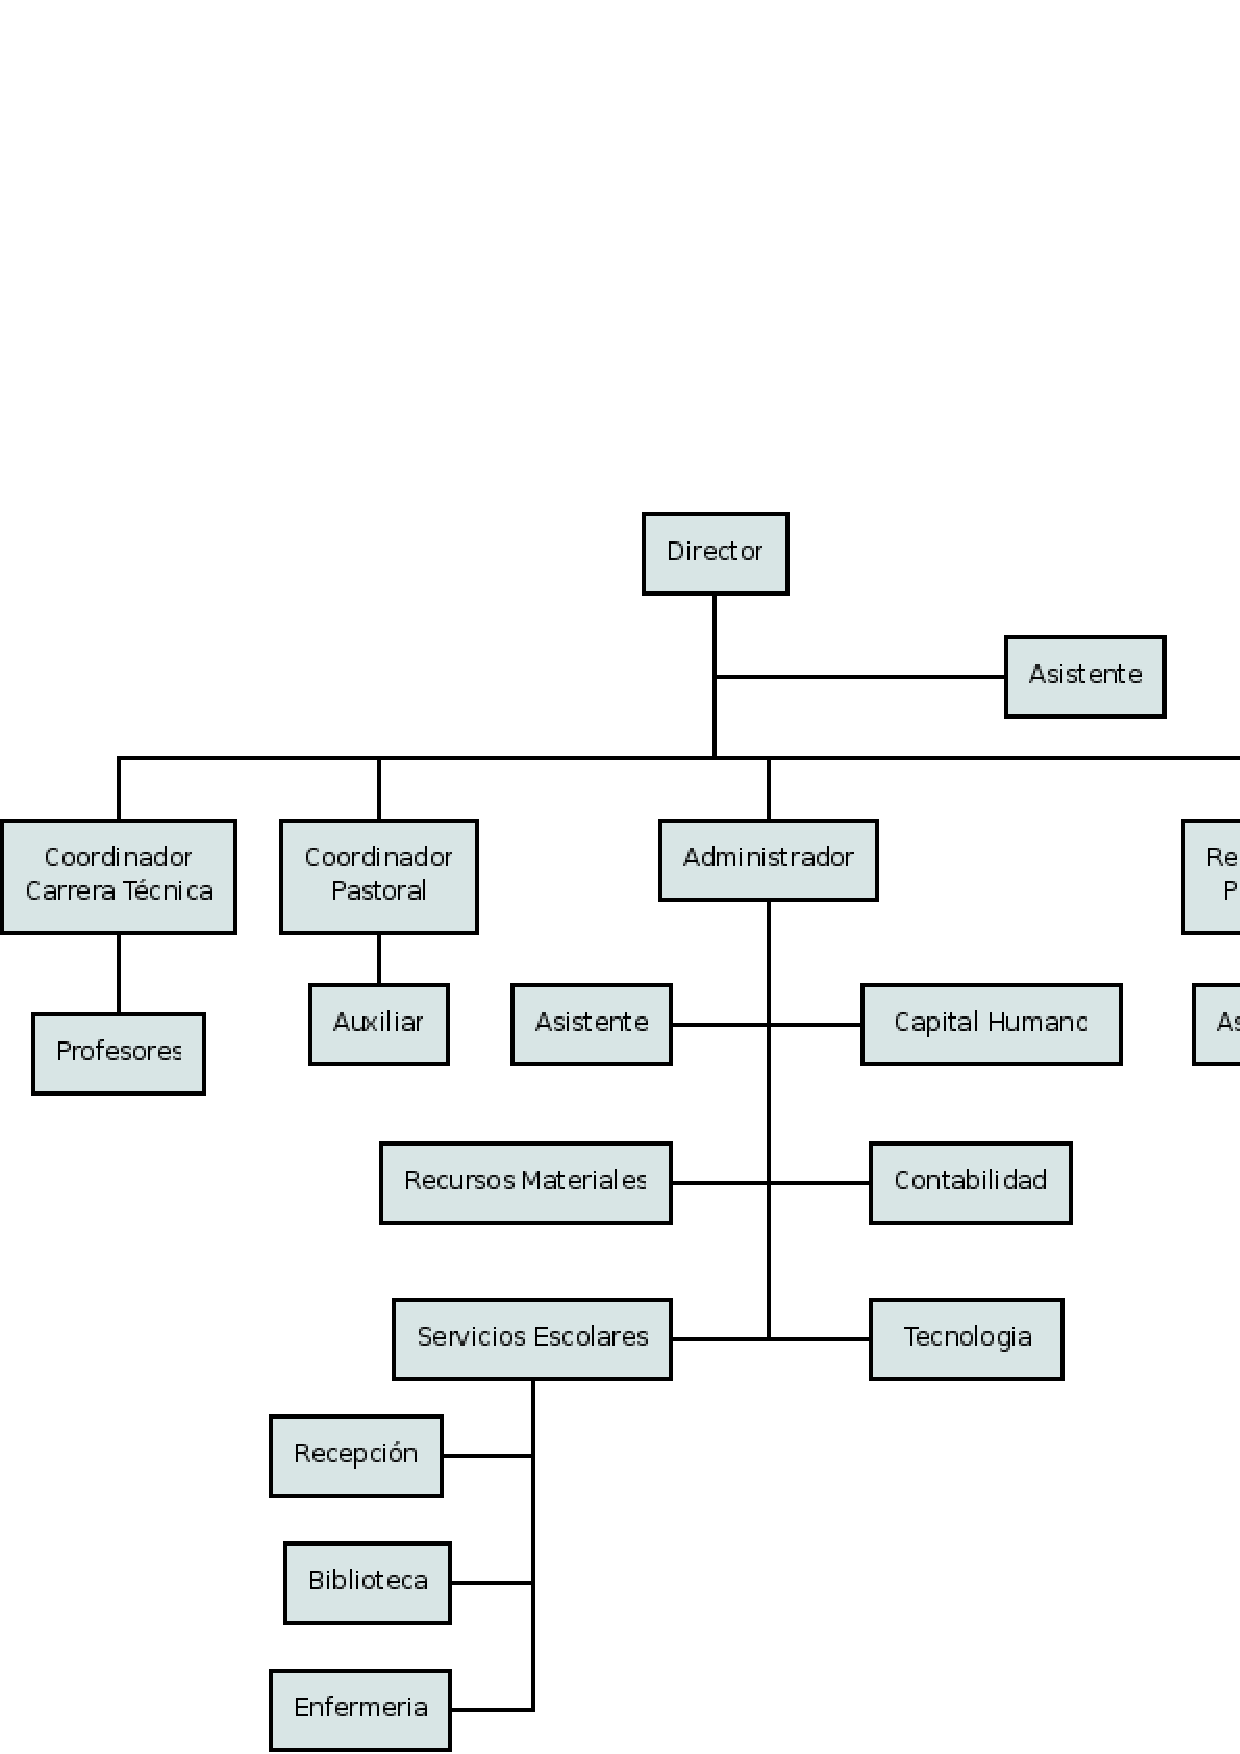
\includegraphics[scale=0.7]{images/organigrama-final}
	\caption[Organigrama Final]{Organigrama Final. Fuente: Elaboración Propia, 2010.}
	\label{fig:Org:Final}
\end{figure}

\begin{figure}
	\centering
	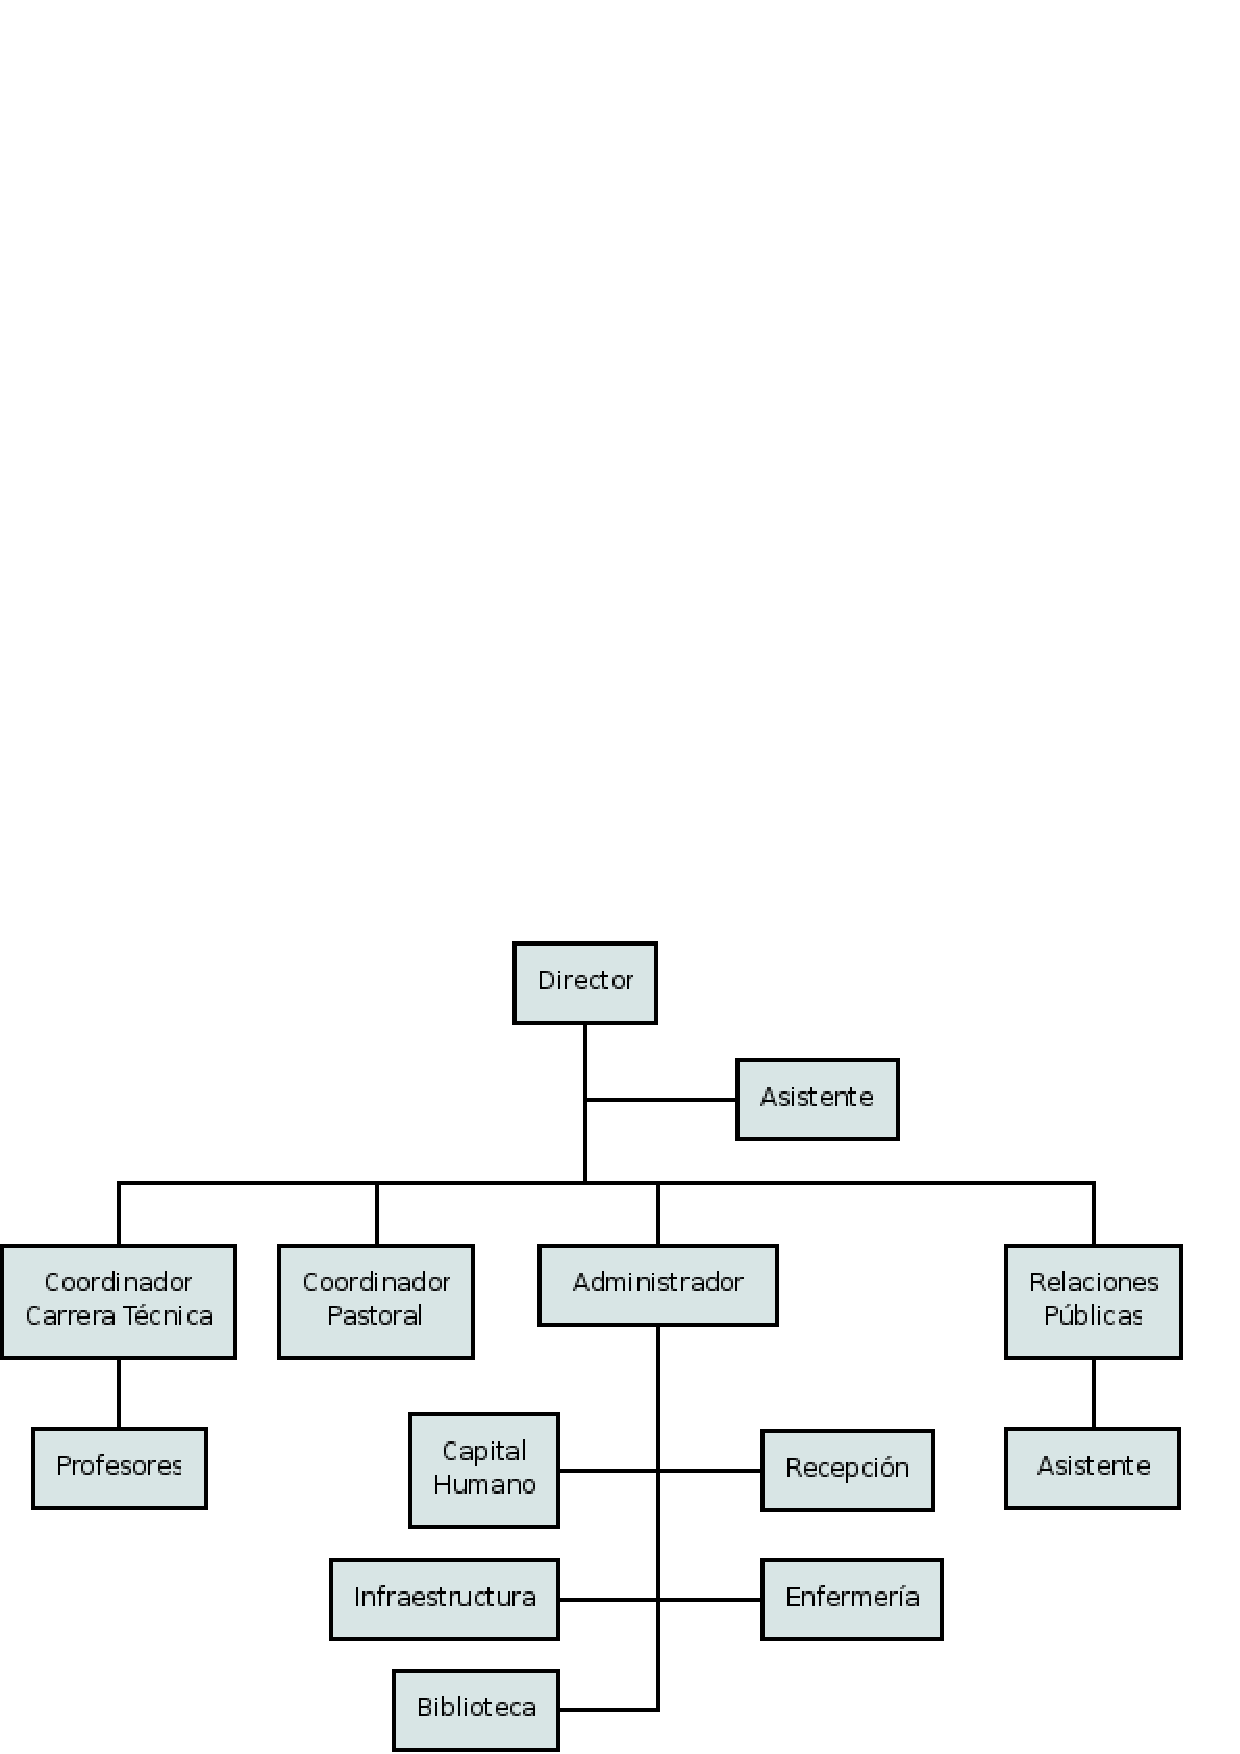
\includegraphics[scale=0.7]{images/organigrama-inicial}
	\caption[Organigrama Inicial]{Organigrama Inicial. Fuente: Elaboración Propia, 2010.}
	\label{fig:Org:Inicial}
\end{figure}

\begin{table}[h]
    \centering
    \caption{Tabla de Sueldos por Cargo}
    \label{tbl:Org:Sueldos}
    \footnotesize
    \begin{tabular}{l|c|c|r|r}
                & \multicolumn{1}{c|}{CANTIDAD}
                & \multicolumn{1}{c|}{CANTIDAD}
                & \multicolumn{1}{c|}{SUELDO}
                & \multicolumn{1}{c}{SUELDO} \\
        \multicolumn{1}{c|}{CARGO}
                & \multicolumn{1}{c|}{INICIAL}
                & \multicolumn{1}{c|}{FINAL}
                & \multicolumn{1}{c|}{INICIAL$^{/a}$}
                & \multicolumn{1}{c}{MENSUAL$^{/b}$} \\
        \hline
        \hline
        Director General                 & 1 &  1 & \$ 21,000.00 & \$ 30,000.00 \\
        Coordinador de Carrera Técnica   & 1 &  3 & \$ 17,500.00 & \$ 25,000.00 \\
        Coordinador de Pastoral          & 1 &  1 & \$ 17,500.00 & \$ 25,000.00 \\
        Administrador                    & 1 &  1 & \$ 17,500.00 & \$ 25,000.00 \\
        Relaciones Públicas              & 1 &  1 & \$ 17,500.00 & \$ 25,000.00 \\
        Encargado de Capital Humano      & 1 &  1 & \$ 14,000.00 & \$ 20,000.00 \\
        Encargado de Infraestructura     & 1 &  0 & \$ 14,000.00 &  N/A$^{/c}$  \\
        Encargado de Contabilidad        & 0 &  1 &       N/A    & \$ 20,000.00 \\
        Encargado de Tecnología          & 0 &  1 &       N/A    & \$ 20,000.00 \\
        Encargado de Recursos Materiales & 0 &  1 &       N/A    & \$ 20,000.00 \\
        Encargado de Servicios Escolares & 0 &  1 &       N/A    & \$ 20,000.00 \\
        Asistente de Dirección           & 2 &  3 & \$ 15,000.00 & \$ 15,000.00 \\
        Enfermera                        & 1 &  1 & \$ 15,000.00 & \$ 15,000.00 \\
        Profesor$^{/d}$                  & 8 & 34 & \$ 16,800.00 & \$ 16,800.00 \\
        Auxiliar                         & 0 &  1 & \$ 10,000.00 & \$ 10,000.00 \\
        Biblioteca                       & 1 &  1 & \$  9,000.00 & \$  9,000.00 \\
        Recepcionista                    & 1 &  1 & \$  9,000.00 & \$  9,000.00 \\
        \hline
        \multicolumn{5}{l}{\footnotesize Fuente: Elaboración Propia, 2010.} \\
        \multicolumn{5}{p{5.5in}}{$^{/a}$ 30\% menor con respecto al definitivo durante los primeros dos años} \\
        \multicolumn{5}{p{5.5in}}{$^{/b}$ Calculado en 2010, se considera 2.5\% de inflación anual} \\
        \multicolumn{5}{p{5.5in}}{$^{/c}$ N/A significa que el puesto no se considera en en escenario indicado} \\
        \multicolumn{5}{p{5.5in}}{$^{/d}$ El sueldo de un profesor es de \$120.00 la hora, la cantidad de \$16.800.00 se calcula sobre la base de que un grupo recibe 35 horas de clase a la semana. Las cantidades indicadas de 8 y 34 corresponden al número de grupos}
    \end{tabular}
\end{table}

\clearpage

\subsubsection{Órganos de Representación}

La escuela cuenta con los siguientes órganos de representación:

\begin{description}
	\item[Patronato]
		Es la máxima autoridad de la escuela, a este órgano rinde cuentas el director por los resultados obtenidos. Tiene un presidente a la cabeza, el cual será siempre un miembro de la congregación salesiana.
	\item[Consejo Escolar]
		Se reúnen con el propósito de proponer mejoras a la escuela tanto académicas como estratégicas. A partir de esta información se mejorará el plan estratégico de la institución. El presidente es el director.
	\item[Sociedad de Alumnos]
		Tiene como finalidad representar a los estudiantes ante el consejo escolar, además de realizar diversas tareas de servicio en coordinación con el alumnado. Tiene un presidente y una planilla que son electos por sus compañeros una vez al año.
\end{description}

\begin{figure}[h]
	\centering
	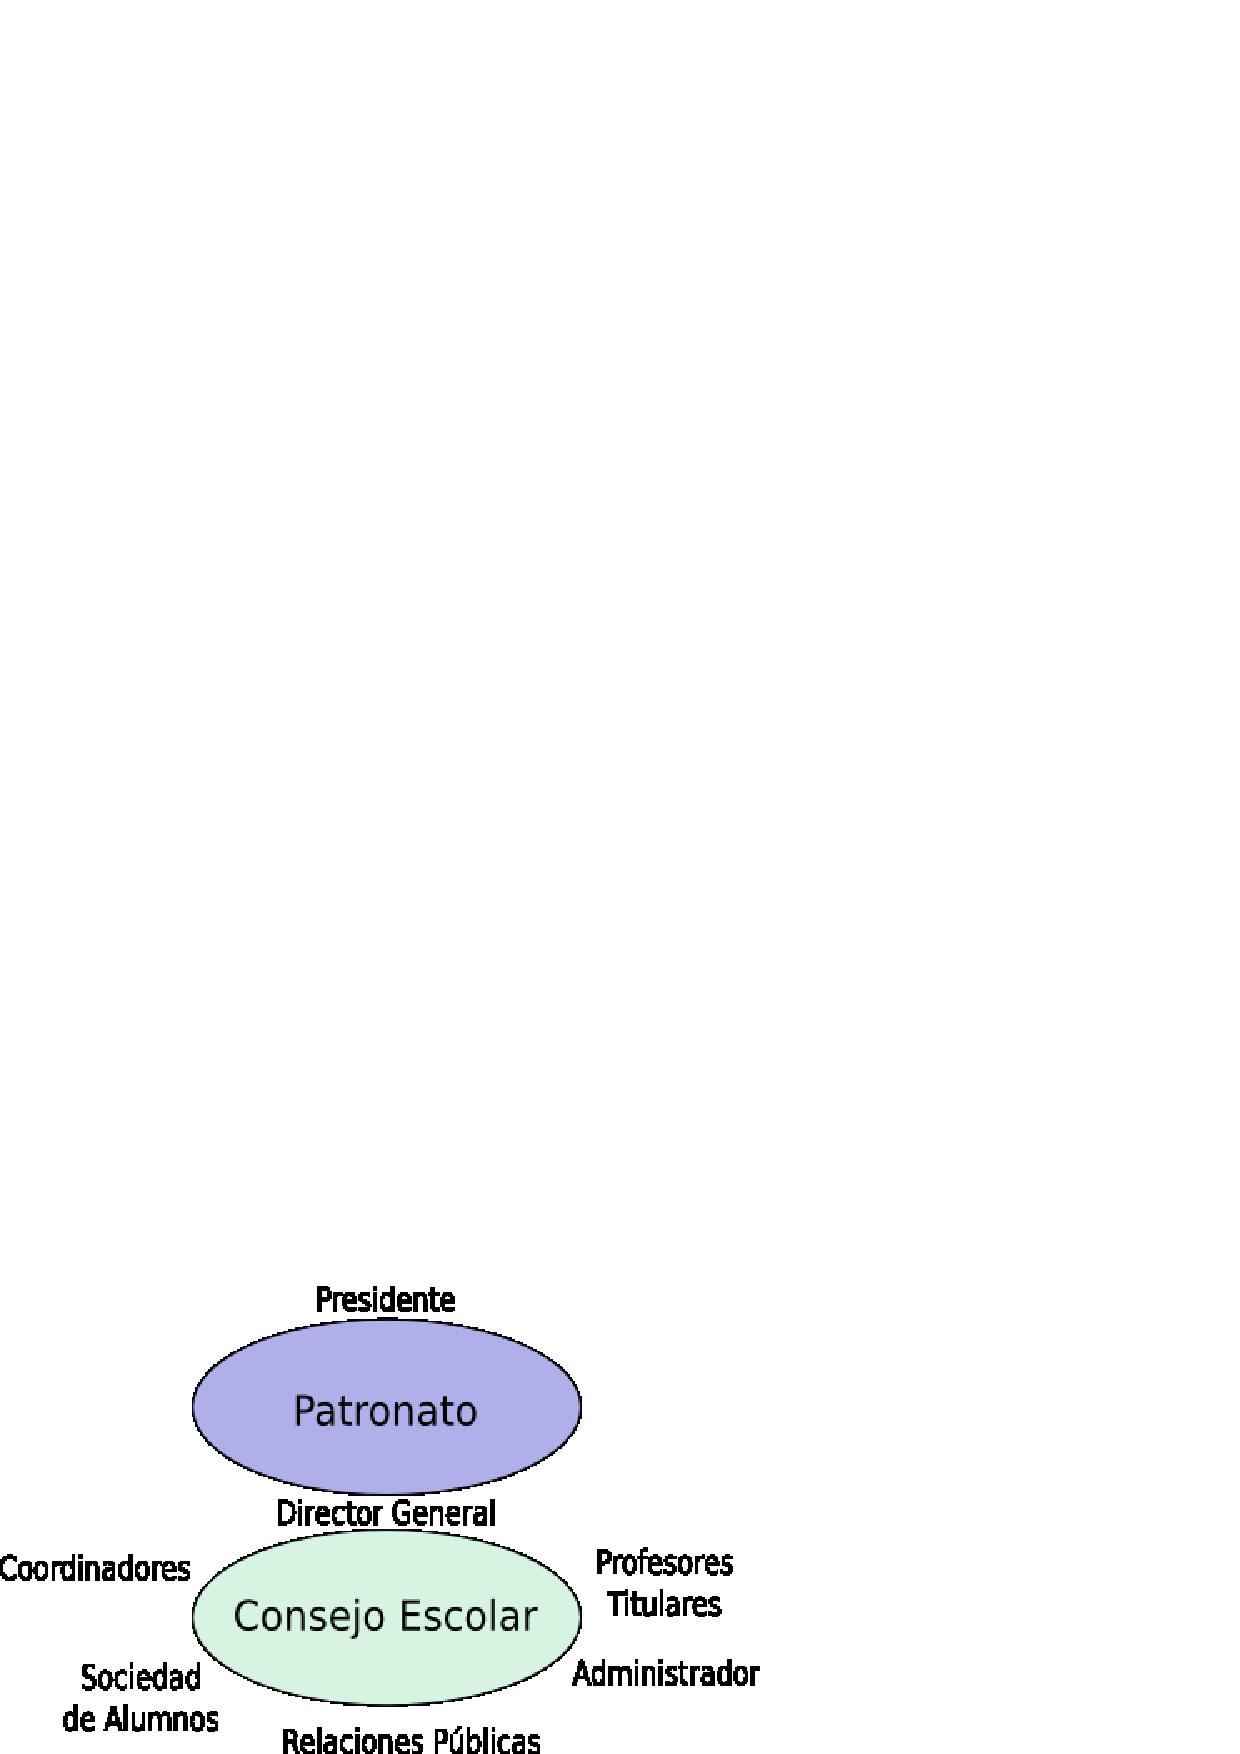
\includegraphics{images/organos}
	\caption[Órganos de Representación]{Órganos de Representación. Fuente: Elaboración Propia, 2010.}
	\label{fig:Org:Organos}
\end{figure}
\clearpage

\section{Aspectos Contables y Legales}

Se consideran dos figuras legales para la constitución de la escuela, en una primera etapa se trata de una Institución de Asistencia Privada (I.A.P.) ya existente: Vida y Esperanza de México, I.A.P.\footnote{\texttt{http://www.enlace.df.gob.mx/busqueda/consultaOsc2.html?b=V}}; la segunda etapa será constituir una Asociación Civil (A.C.) específica para el bachillerato.

La razón de contemplar ambas opciones es la siguiente: la I.A.P. ya existe y goza de prestigio; permite comenzar la labor. La A.C. le dará mayor independencia a la escuela, sin embargo, el reconocimiento oficial toma más de un año.

\subsection{Consideraciones Generales}

La comunidad salesiana en Irapuato, cuenta actualmente con el apoyo de un despacho contable y legal para el cumplimiento de sus obligaciones, especialmente de la fundación Vida y Esperanza de México, I.A.P.; este mismo despacho brindará sus servicios a la escuela en el área de su competencia.

Como parte de los servicios prestados por el despacho, se contemplan las declaraciones fiscales mensuales y anuales. Apoyo durante las auditorías; revisión de contratos laborales y de servicios, litigios, entre otros.

Se consideran los aspectos legales desde dos niveles: federal y local. En el ámbito federal, lo más importante es la autorización de la SEP. El Reconocimiento de Estudios por parte de la autoridad educativa se piensa obtener mediante la figura de extensión de los bachilleratos tecnológicos ya incorporados ante la SEP por parte de otros colegios salesianos.

En el ámbito local, el aspecto más importante a cubrir es el de protección civil. El requisito es tener a una persona que asista a las capacitaciones y después transmita este conocimiento, a la par que se realizan simulacros y se colocan los señalamientos.

\subsection{Vida y Esperanza de México, I.A.P.}

Esta Fundación existe desde hace varios años, cuenta con la autorización de la Secretaría de Hacienda y Crédito Público (S.H.C.P.) para recibir donativos y extender recibos deducibles de impuestos, tiene por objeto social la educación y es presidida por el Pbro. Edmundo Morales Romero, S.D.B.

La principal obligación de la I.A.P. consiste en que cada año es auditada externamente.

\subsection{Una A.C. para el Bachillerato Tecnológico}

Con el propósito de darle independencia legal y financiera a la institución, se tiene pensado crear una A.C. específica; el trámite ante la S.H.C.P. toma de uno a dos años.

En términos generales, una I.A.P. está más acotada por la ley en cuanto a sus funciones y tiene mayor intervención gubernamental tanto en su constitución como en su operación.

Las principales obligaciones de una A.C. son llevar los registros contables y presentar declaraciones mensuales y anuales.

\section{Costos}
\label{sec:Costos}

En una institución educativa, el costo más importante está en los sueldos y salarios; en particular, la nómina de profesores es directamente proporcional al número de estudiantes. Siendo, para este caso, 35 horas por grupo de 30 estudiantes.

La estructura organizacional también aumenta para garantizar el buen orden de las actividades y la coordinación de todos los integrantes de la comunidad.

Para efectos de simplicidad se consideró un profesor de tiempo completo por grupo; sin embargo, en la práctica, la planta docente tiende a ser mucho mayor.

Igualmente, todos los sueldos se colocaron en el rubro de costos fijos, siguiendo el esquema tradicional que se tiene en esta materia.

Como se verá más adelante\footnote{Sección \ref{sec:RecursosColaterales}, página \pageref{sec:RecursosColaterales}.}, se intentará reducir el costo en los diversos rubros mediante patrocinios enfocados.

Un aspecto importante a considerar es la inflación; para este proyecto se consideró de 5\% anual excepto para sueldos, que es de 2.5\% \citep{BANXICO}.

\subsection{Costos Variables}

Los costos variables están conformados por el material de papelería, didáctico y de talleres. El material de talleres representa la parte más importante. Las carreras técnicas específicas que se impartirán tienen pendiente su definición, por tanto, el costo preciso de materiales y maquinaria también. Esta es la razón por la que los costos se estimaron sobre una base genérica por grupo (cuadro \ref{tbl:Costos:Variables}).

\begin{table}
    \centering
    \caption{Costos Variables}
    \label{tbl:Costos:Variables}
    \scriptsize
    \begin{tabular}{l@{\hspace{1mm}}|r*{5}{|@{\hspace{1mm}}c@{\hspace{1mm}}|@{\hspace{1mm}}r@{\hspace{1mm}}}}
		&	PRECIO	&	\multicolumn{2}{c|}{AÑO 1}	&	\multicolumn{2}{c|}{AÑO 2}	&	\multicolumn{2}{c|}{AÑO 3}	&	\multicolumn{2}{c|}{AÑO 4}	&	\multicolumn{2}{c}{AÑO 5} \\
	\cline{3-12}
	\multicolumn{1}{c|}{CONCEPTO}	&	UNITARIO	&	C$^{/a}$	&	\multicolumn{1}{c|}{TOTAL}	&	C	&	\multicolumn{1}{c|}{TOTAL}	&	C	&	\multicolumn{1}{c|}{TOTAL}	&	C	&	\multicolumn{1}{c|}{TOTAL}	&	C	&	\multicolumn{1}{c}{TOTAL} \\
	\hline
	\hline
	PAPELERÍA \\
	\hline
	Hojas (caja con 5000)	&	200.00	&	4	&	892.00	&	9	&	1,869.00	&	13	&	2,941.47	&	18	&	4,121.15	&	20	&	4,862.03 \\
	Bolígrafos (10 pzas)	&	30.00	&	52	&	1,560.00	&	56	&	1,764.00	&	72	&	2,381.40	&	72	&	2,500.47	&	72	&	2,625.49 \\
	Tóner (2 pzas)	&	2,000.00	&	4	&	8,920.00	&	9	&	18,690.00	&	13	&	29,414.70	&	18	&	41,211.45	&	20	&	48,620.25 \\
	Carpetas (pza.)	&	50.00	&	20	&	1,000.00	&	20	&	1,050.00	&	20	&	1,102.50	&	20	&	1,157.63	&	20	&	1,215.51 \\
	\hline
	SUBTOTAL	&		&		&	12,372.00	&		&	23,373.00	&		&	35,840.07	&		&	48,990.69	&		&	57,323.27 \\
	\hline
	MATERIAL DIDÁCTICO \\
	\hline
	Plumones (4 pzas.)	&	50.00	&	240	&	12,000.00	&	450	&	23,625.00	&	690	&	38,036.25	&	900	&	52,093.13	&	1,020	&	61,990.82 \\
	Borradores (pza.)	&	30.00	&	48	&	1,440.00	&	90	&	2,835.00	&	138	&	4,564.35	&	180	&	6,251.18	&	204	&	7,438.90 \\
	\hline
	SUBTOTAL	&		&		&	13,440.00	&		&	26,460.00	&		&	42,600.60	&		&	58,344.30	&		&	69,429.72 \\
	\hline
	MATERIAL TALLERES \\
	\hline
	Material talleres$^{/b}$	&	5,000.00	&	7	&	35,000.00	&	14	&	73,500.00	&	18	&	99,225.00	&	24	&	138,915.00	&	30	&	182,325.94 \\
	\hline
	SUBTOTAL	&		&		&	35,000.00	&		&	73,500.00	&		&	99,225.00	&		&	138,915.00	&		&	182,325.94 \\
	\hline
	\hline
	TOTAL	&		&		&	60,812.00	&		&	123,333.00	&		&	177,665.67	&		&	246,249.99	&		&	309,078.93 \\
	\hline
	\multicolumn{12}{l}{\footnotesize Fuente: Elaboración Propia, 2010.} \\
	\multicolumn{12}{l}{$^{/a}$ Cantidad} \\
	\multicolumn{12}{l}{$^{/b}$ Material para un grupo de 30 estudiantes} \\
    \end{tabular}
\end{table}


\subsection{Costos Fijos}

El cuadro \ref{tbl:Costos:Fijos} muestra los costos fijos, éstos se integran por los servicios subcontratados (vigilancia, limpieza, etc.), los de infraestructura (agua, luz, etc.), las actividades de promoción (publicidad) y la nómina en sus diferentes niveles.

Para el caso de los servicios subcontratados de vigilancia y limpieza se consideró como unidad el sueldo/mes/hombre. En el caso del despacho contable y legal, una anualidad. Para los servicios de infraestructura (agua, luz, teléfono con internet) se calculó una anualidad mediante la interpolación sobre el estado de resultados de un colegio de menor tamaño en Irapuato\footnote{Uno de los interesados en el proyecto trabaja como administrativo de un bachillerato de pequeño tamaño, fue quien aportó los estados de resultados de su centro de trabajo.}.

\begin{table}
    \centering
    \caption{Costos Fijos}
    \label{tbl:Costos:Fijos}
    \scriptsize
    \begin{tabular}{l@{\hspace{1mm}}|r*{5}{|@{\hspace{1mm}}c@{\hspace{1mm}}|@{\hspace{1mm}}r@{\hspace{1mm}}}}
		&	PRECIO	&	\multicolumn{2}{c|}{AÑO 1}	&	\multicolumn{2}{c|}{AÑO 2}	&	\multicolumn{2}{c|}{AÑO 3}	&	\multicolumn{2}{c|}{AÑO 4}	&	\multicolumn{2}{c}{AÑO 5} \\
	\cline{3-12}
	\multicolumn{1}{c|}{CONCEPTO}	&	UNITARIO	&	C$^{/a}$	&	\multicolumn{1}{c|}{TOTAL}	&	C	&	\multicolumn{1}{c|}{TOTAL}	&	C	&	\multicolumn{1}{c|}{TOTAL}	&	C	&	\multicolumn{1}{c|}{TOTAL}	&	C	&	\multicolumn{1}{c}{TOTAL} \\
	\hline
	\hline
	\multicolumn{12}{l}{SERVICIOS SUBCONTRATADOS} \\
	\hline
	Vigilancia	&	8,000.00	&	72	&	576,000.00	&	72	&	604,800.00	&	72	&	635,040.00	&	72	&	666,792.00	&	72	&	700,131.60 \\
	Limpieza	&	5,000.00	&	40	&	200,000.00	&	40	&	210,000.00	&	40	&	220,500.00	&	40	&	231,525.00	&	40	&	243,101.25 \\
	Despacho legal$^{/b}$	&	60,000.00	&	1	&	60,000.00	&	12	&	756,000.00	&	12	&	793,800.00	&	12	&	833,490.00	&	12	&	875,164.50 \\
	\hline
	SUBTOTAL	&		&		&	836,000.00	&		&	1,570,800.00	&		&	1,649,340.00	&		&	1,731,807.00	&		&	1,818,397.35 \\
	\hline
	\multicolumn{12}{l}{SERVICIOS DE INFRAESTRUCTURA} \\
	\hline
	Luz	&	300,000.00	&	1	&	300,000.00	&	1	&	315,000.00	&	1	&	330,750.00	&	1	&	347,287.50	&	1	&	364,651.88 \\
	Teléfono	&	120,000.00	&	1	&	120,000.00	&	1	&	126,000.00	&	1	&	132,300.00	&	1	&	138,915.00	&	1	&	145,860.75 \\
	Agua	&	100,000.00	&	1	&	100,000.00	&	1	&	105,000.00	&	1	&	110,250.00	&	1	&	115,762.50	&	1	&	121,550.63 \\
	\hline
	SUBTOTAL	&		&		&	520,000.00	&		&	546,000.00	&		&	573,300.00	&		&	601,965.00	&		&	632,063.25 \\
	\hline
	\multicolumn{12}{l}{PROMOCIÓN} \\
	\hline
	Publicidad	&	15,000.00	&	12	&	180,000.00	&	12	&	189,000.00	&	12	&	198,450.00	&	12	&	208,372.50	&	12	&	218,791.13 \\
	\hline
	SUBTOTAL	&		&		&	180,000.00	&		&	189,000.00	&		&	198,450.00	&		&	208,372.50	&		&	218,791.13 \\
	\hline
	\multicolumn{12}{l}{SUELDOS$^{/c}$} \\
	\hline
	Sueldos Directos	&		&		&	2,070,750.24	&		&	3,760,368.30	&		&	5,915,755.70	&		&	7,784,415.02	&		&	8,986,902.29 \\
	Sueldos Indirectos	&		&		&	1,195,708.80	&		&	1,225,601.52	&		&	2,284,075.56	&		&	2,341,177.45	&		&	2,399,706.89 \\
	Sueldos	&		&		&	1,236,471.60	&		&	1,511,110.97	&		&	2,569,585.01	&		&	2,633,824.63	&		&	2,699,670.25 \\
	 Administrativos &&&&&&&&&&\\
		\hline
	SUBTOTAL	&		&		&	4,502,930.64	&		&	6,497,080.79	&		&	10,769,416.27	&		&	12,759,417.10	&		&	14,086,279.42 \\
	\hline
	\hline
	TOTAL	&		&		&	6,038,930.64	&		&	8,802,880.79	&		&	13,190,506.27	&		&	15,301,561.60	&		&	16,755,531.14 \\
	\hline
	\multicolumn{12}{l}{\footnotesize Fuente: Elaboración Propia, 2010.} \\
	\multicolumn{12}{l}{$^{/a}$ Cantidad} \\
	\multicolumn{12}{l}{$^{/b}$ Despacho legal y contable} \\
	\multicolumn{12}{l}{$^{/c}$ El detalle sobre los sueldos se muestra en los cuadros \ref{tbl:Sueldos:Detalle:1} y \ref{tbl:Sueldos:Detalle:2}} \\
    \end{tabular}
\end{table}


\begin{table}
    \caption{Detalle de Sueldos}
    \label{tbl:Sueldos:Detalle:1}
    \centering
    \scriptsize
    \begin{tabular}{l@{\hspace{1mm}}|@{\hspace{1mm}}r@{\hspace{1mm}}|@{\hspace{1mm}}r*{3}{|@{\hspace{1mm}}c@{\hspace{1mm}}|@{\hspace{1mm}}r@{\hspace{1mm}}}}
                &	SUELDO	&	SUELDO	&	\multicolumn{2}{c|}{AÑO 1}	&	\multicolumn{2}{c|}{AÑO 2}	&	\multicolumn{2}{c}{AÑO 3} \\
    \cline{4-9}
        PUESTO	&	SIMPLE$^{/a}$	&	INTEGRADO$^{/a}$	&	C$^{/c}$	&	\multicolumn{1}{c|}{TOTAL}	&	C	&	\multicolumn{1}{c|}{TOTAL}	&	C	&	\multicolumn{1}{c}{TOTAL} \\
%--------------------------------------------------
	\hline
	\hline
	\multicolumn{9}{l}{SUELDOS DIRECTOS} \\
	\hline
	Auxiliar pastoral	&2,500.00		&	2,613.00	&	0	&	0.00	&	0	&	0.00	&	1	&	142,754.72 \\
	Profesor		&4,200.00	&	4,389.84	&	8	&	1,826,173.44	&	15	&	3,509,677.08	&	23	&	5,516,042.48 \\
	Recepción		&2,250.00	&	2,351.70	&	1	&	122,288.40	&	1	&	125,345.61	&	1	&	128,479.25 \\
	Biblioteca		&2,250.00	&	2,351.70	&	1	&	122,288.40	&	1	&	125,345.61	&	1	&	128,479.25 \\

	\hline
	\multicolumn{2}{l}{} & TOTAL: &	\multicolumn{1}{l}{}	&	2,070,750.24	&	\multicolumn{1}{l}{}	&	3,760,368.30	&	\multicolumn{1}{l}{}	&	5,915,755.70 \\
%--------------------------------------------------
	\hline
	\hline
	\multicolumn{9}{l}{SUELDOS INDIRECTOS} \\
	\hline
	Enfermería                   &	3,750.00	&	3,919.50	&	1	&	203,814.00	&	1	&	208,909.35	&	1	&	214,132.08 \\
	Asistente                    &	3,750.00	&	3,919.50	&	3	&	611,442.00	&	3	&	626,728.05	&	3	&	642,396.25 \\
	Capital Humano Etapa Inicial &	3,500.00	&	3,658.20	&	1	&	190,226.40	&	1	&	194,982.06	&	0	&	0.00 \\
	Infraestructura Etapa Inicial       &	3,500.00	&	3,658.20	&	1	&	190,226.40	&	1	&	194,982.06	&	0	&	0.00 \\
	Capital Humano               &	5,000.00	&	5,226.00	&	0	&	0.00	&	0	&	0.00	&	1	&	285,509.45 \\
	Contabilidad                 &	5,000.00	&	5,226.00	&	0	&	0.00	&	0	&	0.00	&	1	&	285,509.45 \\
	Tecnología                   &	5,000.00	&	5,226.00	&	0	&	0.00	&	0	&	0.00	&	1	&	285,509.45 \\
	Recursos Materiales          &	5,000.00	&	5,226.00	&	0	&	0.00	&	0	&	0.00	&	1	&	285,509.45 \\
	Servicios Escolares          &	5,000.00	&	5,226.00	&	0	&	0.00	&	0	&	0.00	&	1	&	285,509.45 \\
	\hline
	\multicolumn{2}{l}{} & TOTAL: &
	    \multicolumn{1}{l}{} & 1,195,708.80 &
	    \multicolumn{1}{l}{} & 1,225,601.52 &
	    \multicolumn{1}{l}{} & 2,284,075.56 \\
%--------------------------------------------------
	\hline
	\hline
	\multicolumn{9}{l}{SUELDOS ADMINISTRATIVOS} \\
	\hline
	Director Etapa Inicial                    &	5,250.00	&	5,487.30	&	1	&	285,339.60	&	1	&	292,473.09	&	0	&	0.00 \\
	Coordinador Carrera Técnica Etapa Inicial &	4,375.00	&	4,572.75	&	1	&	237,783.00	&	2	&	487,455.15	&	0	&	0.00 \\
	Coordinador Pastoral Etapa Inicial        &	4,375.00	&	4,572.75	&	1	&	237,783.00	&	1	&	243,727.58	&	0	&	0.00 \\
	Administrador Etapa Inicial               &	4,375.00	&	4,572.75	&	1	&	237,783.00	&	1	&	243,727.58	&	0	&	0.00 \\
	Relaciones Públicas Etapa Inicial         &	4,375.00	&	4,572.75	&	1	&	237,783.00	&	1	&	243,727.58	&	0	&	0.00 \\
	Director                         &	7,500.00	&	7,839.00	&	0	&	0.00	&	0	&	0.00	&	1	&	428,264.17 \\
	Coordinador Carrera Técnica      &	6,250.00	&	6,532.50	&	0	&	0.00	&	0	&	0.00	&	3	&	1,070,660.42 \\
	Coordinador Pastoral             &	6,250.00	&	6,532.50	&	0	&	0.00	&	0	&	0.00	&	1	&	356,886.81 \\
	Administrador                    &	6,250.00	&	6,532.50	&	0	&	0.00	&	0	&	0.00	&	1	&	356,886.81 \\
	Relaciones Públicas              &	6,250.00	&	6,532.50	&	0	&	0.00	&	0	&	0.00	&	1	&	356,886.81 \\
	\hline
	\multicolumn{2}{l}{} & TOTAL: &
	    \multicolumn{1}{l}{} & 1,236,471.60 &
	    \multicolumn{1}{l}{} & 1,511,110.97 &
	    \multicolumn{1}{l}{} & 2,569,585.01 \\
%--------------------------------------------------
	\hline
	\multicolumn{9}{l}{\footnotesize Fuente: Elaboración Propia, 2010.} \\
	\multicolumn{9}{l}{$^{/a}$ Sueldo Semanal Simple} \\
	\multicolumn{9}{l}{$^{/b}$ Sueldo Semanal Integrado} \\
	\multicolumn{9}{l}{$^{/c}$ Cantidad} \\
    \end{tabular}
\end{table}


\begin{table}
    \caption{Detalle de Sueldos (continuación)}
    \label{tbl:Sueldos:Detalle:2}
    \centering
    \scriptsize
    \begin{tabular}{l@{\hspace{1mm}}|@{\hspace{1mm}}r@{\hspace{1mm}}|@{\hspace{1mm}}r*{2}{|@{\hspace{1mm}}c@{\hspace{1mm}}|@{\hspace{1mm}}r@{\hspace{1mm}}}}
                &	SUELDO	&	SUELDO	&	\multicolumn{2}{c|}{AÑO 4}	&	\multicolumn{2}{c}{AÑO 5} \\
    \cline{4-7}
        PUESTO	&	SIMPLE$^{/a}$	&	INTEGRADO$^{/a}$	&	C	&	\multicolumn{1}{c|}{TOTAL}	&	C	&	\multicolumn{1}{c}{TOTAL} \\
%--------------------------------------------------
	\hline
	\hline
	\multicolumn{7}{l}{SUELDOS DIRECTOS} \\
	\hline
	Auxiliar pastoral	&2,500.00		&	2,613.00	&	1	&	146,323.59	&	1	&	149,981.68 \\
	Profesor		&4,200.00		&	4,389.84	&	30	&	7,374,708.96	&	34	&	8,566,953.58 \\
	Recepción		&2,250.00		&	2,351.70	&	1	&	131,691.23	&	1	&	134,983.51 \\
	Biblioteca		&2,250.00		&	2,351.70	&	1	&	131,691.23	&	1	&	134,983.51 \\

	\hline
	\multicolumn{2}{l}{} & TOTAL: &
		\multicolumn{1}{l}{}	&	7,784,415.02	&
		\multicolumn{1}{l}{}	&	8,986,902.29 \\
%--------------------------------------------------
	\hline
	\hline
	\multicolumn{7}{l}{SUELDOS INDIRECTOS} \\
	\hline
	Enfermeria                   &	3,750.00	&	3,919.50	&	1	&	219,485.39	&	1	&	224,972.52 \\
	Asistente                    &	3,750.00	&	3,919.50	&	3	&	658,456.16	&	3	&	674,917.56 \\
	Capital Humano Etapa Inicial &	3,500.00	&	3,658.20	&	0	&	0.00	&	0	&	0.00 \\
	Infraestructura Etapa Inicial       &	3,500.00	&	3,658.20	&	0	&	0.00	&	0	&	0.00 \\
	Capital Humano               &	5,000.00	&	5,226.00	&	1	&	292,647.18	&	1	&	299,963.36 \\
	Contabilidad                 &	5,000.00	&	5,226.00	&	1	&	292,647.18	&	1	&	299,963.36 \\
	Tecnología                   &	5,000.00	&	5,226.00	&	1	&	292,647.18	&	1	&	299,963.36 \\
	Recursos Materiales          &	5,000.00	&	5,226.00	&	1	&	292,647.18	&	1	&	299,963.36 \\
	Servicios Escolares          &	5,000.00	&	5,226.00	&	1	&	292,647.18	&	1	&	299,963.36 \\
	\hline
	\multicolumn{2}{l}{} & TOTAL: &
	    \multicolumn{1}{l}{} & 2,341,177.45 &
	    \multicolumn{1}{l}{} & 2,399,706.89 \\
%--------------------------------------------------
	\hline
	\hline
	\multicolumn{7}{l}{SUELDOS ADMINISTRATIVOS} \\
	\hline
	Director Etapa Inicial                    &	5,250.00	&	5,487.30	&	0	&	0.00	&	0	&	0.00 \\
	Coordinador Carrera Técnica Etapa Inicial &	4,375.00	&	4,572.75	&	0	&	0.00	&	0	&	0.00 \\
	Coordinador Pastoral Etapa Inicial        &	4,375.00	&	4,572.75	&	0	&	0.00	&	0	&	0.00 \\
	Administrador Etapa Inicial               &	4,375.00	&	4,572.75	&	0	&	0.00	&	0	&	0.00 \\
	Relaciones Públicas Etapa Inicial         &	4,375.00	&	4,572.75	&	0	&	0.00	&	0	&	0.00 \\
	Director                         &	7,500.00	&	7,839.00	&	1	&	438,970.77	&	1	&	449,945.04 \\
	Coordinador Carrera Técnica      &	6,250.00	&	6,532.50	&	3	&	1,097,426.93	&	3	&	1,124,862.60 \\
	Coordinador Pastoral             &	6,250.00	&	6,532.50	&	1	&	365,808.98	&	1	&	374,954.20 \\
	Administrador                    &	6,250.00	&	6,532.50	&	1	&	365,808.98	&	1	&	374,954.20 \\
	Relaciones Públicas              &	6,250.00	&	6,532.50	&	1	&	365,808.98	&	1	&	374,954.20 \\
	\hline
	\multicolumn{2}{l}{} & TOTAL: &
	    \multicolumn{1}{l}{} & 2,633,824.63 &
	    \multicolumn{1}{l}{} & 2,699,670.25 \\
%--------------------------------------------------
	\hline
	\multicolumn{7}{l}{\footnotesize Fuente: Elaboración Propia, 2010.} \\
	\multicolumn{7}{l}{$^{/a}$ Sueldo Semanal Simple} \\
	\multicolumn{7}{l}{$^{/b}$ Sueldo Semanal Integrado} \\
	\multicolumn{7}{l}{$^{/c}$ Cantidad} \\
    \end{tabular}
\end{table}


\clearpage
\section{Presupuestos}

Un presupuesto es el cálculo anticipado de los ingresos y gastos de una actividad económica durante un periodo, por lo general anual. Es un plan de acción dirigido a cumplir una meta prevista expresada en términos financieros.

Los presupuestos de este proyecto se clasifican en los siguientes tres rubros:

\begin{itemize}
	\item Presupuesto de ingresos (proyección de ventas).
	\item Inversión inicial.
	\item Presupuesto de egresos.
\end{itemize}

\subsection{Proyección de Ventas}

Considerando una colegiatura base de \$ 3,000.00 se considera un porcentaje de becas distinto para cada escenario, siendo para el escenario pesimista de 20\%, 30\% para el escenario intermedio y 40\% en el escenario idealista. El objetivo es ofrecer una mayor cobertura de becas a medida que la matrícula estudiantil aumenta pues es un proyecto que busca atender a los más necesitados (cuadros \ref{tbl:ProyeccionIngreso} y \ref{tbl:ProyeccionIngreso:Anual} y figura \ref{fig:ProyeccionIngresos}).\footnote{El porcentaje de becas se incluye en los cálculos mediante su aplicación al monto de la colegiatura \emph{como si se aplicara a la totalidad del alumnado}, sin embargo, la forma concreta de distribuir las becas entre la población estudiantil es materia pendiente de discusión y escapa al alcance de este trabajo; para mayor información revisar el capítulo \ref{ch:Introduccion} (\nameref{ch:Introduccion}) a partir de la página \pageref{ch:Introduccion} para más detalles al respecto.}

\begin{table}[h]
    \centering
    \caption{Proyecci\'on del Ingreso para los Primeros Cinco Años\newline (Ingreso Mensual)}
    \label{tbl:ProyeccionIngreso}
    %\footnotesize
    \begin{tabular}{l|r|r|r|r|r|r}
        \multicolumn{2}{c|}{}
            & \multicolumn{5}{c}{Ingresos mensuales por concepto de colegiaturas$^{/a}$} \\
        \cline{3-7}
        \multicolumn{2}{c|}{}
            & \multicolumn{1}{c|}{AÑO 1}
            & \multicolumn{1}{c|}{AÑO 2}
            & \multicolumn{1}{c|}{AÑO 3}
            & \multicolumn{1}{c|}{AÑO 4}
            & \multicolumn{1}{c }{AÑO 5} \\
        ESCENARIO
            & PRECIO
            & \multicolumn{1}{c|}{(33 \%) }
            & \multicolumn{1}{c|}{(67 \%) }
            & \multicolumn{1}{c|}{(100 \%)}
            & \multicolumn{1}{c|}{(100 \%)}
            & \multicolumn{1}{c }{(100 \%)} \\
        \hline
        \hline
        Optimista
            & \$ 1,800.00   % cupo, precio
            & \$ 600.0      % año 1
            & \$ 1,200.0    % año 2
            & \$ 1,800.0    % año 3
            & \$ 1,800.0    % año 4
            & \$ 1,800.0 \\ % año 5
        \hline
        Intermedio
            & \$ 2,100.00   % cupo, precio
            & \$   466.9    % año 1
            & \$   933.8    % año 2
            & \$ 1,400.7    % año 3
            & \$ 1,602.0    % año 4
            & \$ 1,800.0 \\ % año 5
        \hline
        Pesimista
            & \$ 2,400.00 % cupo, precio
            & \$   264.0    % año 1
            & \$   528.0    % año 2
            & \$   792.0    % año 3
            & \$ 1,050.0    % año 4
            & \$ 1,400.7 \\ % año 5
        \hline
        \multicolumn{7}{l}{\footnotesize Fuente: Elaboración Propia, 2010.} \\
        \multicolumn{7}{l}{\footnotesize $^{/a}$ Miles de pesos.}
    \end{tabular}
\end{table}



\begin{table}
    \centering
    \caption{Proyecci\'on del Ingreso para los Primeros Cinco Años\newline (Ingreso Anual)}
    \label{tbl:ProyeccionIngreso:Anual}
    %\footnotesize
    \begin{tabular}{l*{5}{|r}}
        \multicolumn{1}{c|}{}
            & \multicolumn{5}{c}{Ingresos anuales por concepto de colegiaturas$^{/a}$} \\
        \cline{2-6}
        \multicolumn{1}{c|}{}
            & \multicolumn{1}{c|}{AÑO 1}
            & \multicolumn{1}{c|}{AÑO 2}
            & \multicolumn{1}{c|}{AÑO 3}
            & \multicolumn{1}{c|}{AÑO 4}
            & \multicolumn{1}{c }{AÑO 5} \\
        ESCENARIO
            & \multicolumn{1}{c|}{(33 \%) }
            & \multicolumn{1}{c|}{(67 \%) }
            & \multicolumn{1}{c|}{(100 \%)}
            & \multicolumn{1}{c|}{(100 \%)}
            & \multicolumn{1}{c }{(100 \%)} \\
        \hline
        \hline
        Optimista
            & \$  7,200.0 % año 1
            & \$ 14,400.0 % año 2
            & \$ 21,600.0 % año 3
            & \$ 21,600.0 % año 4
            & \$ 21,600.0 \\ % año 5
        \hline
        Intermedio
            & \$  5,602.8 % año 1
            & \$ 11,205.6 % año 2
            & \$ 16,808.4 % año 3
            & \$ 19,224.0 % año 4
            & \$ 21,600.0 \\ % año 5
        \hline
        Pesimista
            & \$  3,168.0 % año 1
            & \$  6,336.0 % año 2
            & \$  9,504.0 % año 3
            & \$ 12,600.0 % año 4
            & \$ 16,808.4 \\ % año 5
        \hline
        \multicolumn{6}{l}{\footnotesize Fuente: Elaboración Propia, 2010.} \\
        \multicolumn{6}{l}{\footnotesize $^{/a}$ Miles de pesos.}
    \end{tabular}
\end{table}



\begin{figure}
	\centering
	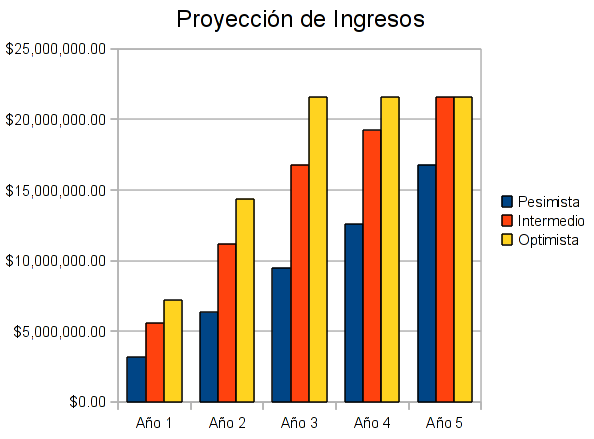
\includegraphics[scale=0.7]{images/proyeccion_ingresos}
	\caption[Proyecci\'on del Ingreso para los Primeros Cinco Años]{Proyecci\'on del Ingreso para los Primeros Cinco Años\newline (Ingreso Anual). Fuente: Elaboración Propia, 2010.}
	\label{fig:ProyeccionIngresos}
\end{figure}

\subsection{Inversión Inicial}
\label{sub:oper:InversionInicial}

La inversión inicial está compuesta por el activo fijo y el activo circulante necesario para operar; el activo circulante inicial contiene el costo de inicio de proyecto (\$951,675.00)\footnote{Ver la subsección \ref{sub:Proy:Costo}, página \pageref{sub:Proy:Costo}. Los costos del proyecto se dividen en dos: los montos para remodelación y material inicial se incluyen en la inversión en activo fijo y los sueldos y honorarios del proyecto en el activo circulante inicial.} y una cantidad inicial de becas que se considera en \$1,000,000.00.

Se espera obtener un patrocinio inicial de \$3,000.000.00 y un crédito bancario por \$2,308,390.00. Además, se tiene intención de renovar la infraestructura (activo fijo) a lo largo del tiempo. En total, la inversión inicial es de \$ 11,579,099.40 (ver cuadro \ref{tbl:InversionInicial})

\begin{table}[h]
    \caption{Inversión Inicial}
    \label{tbl:InversionInicial}
    \centering
    \footnotesize
    \begin{tabular}{l*{6}{|r}}
	    &	\multicolumn{5}{c}{Inversiones}	& \\
	\cline{2-7}
	\multicolumn{1}{c|}{CONCEPTO}	&	\multicolumn{1}{c|}{AÑO 1}	&	\multicolumn{1}{c|}{AÑO 2}	&	\multicolumn{1}{c|}{AÑO 3}	&	\multicolumn{1}{c|}{AÑO 4}	&	\multicolumn{1}{c|}{AÑO 5}	&	\multicolumn{1}{c}{TOTAL} \\
	\hline
	\hline
	Activo Circulante	&	2,903,350.00	&	0.00	&	0.00	&	0.00	&	0.00	&	2,903,350.00 \\
	Activos Fijos	&	7,792,599.40	&	100,000.00	&	303,150.00	&	480,000.00	&	0.00	&	8,675,749.40 \\
	Activos diferidos$^{/a}$	&	0.00	&	0.00	&	0.00	&	0.00	&	0.00	&	0.00 \\
	\hline
	TOTAL	&	10,695,949.40	&	100,000.00	&	303,150.00	&	480,000.00	&	0.00	&	11,579,099.40 \\
	\hline
	\multicolumn{7}{l}{\footnotesize Fuente: Elaboración Propia, 2010.} \\
	\multicolumn{7}{l}{$^{/a}$ Ver la subsección \ref{sub:Otros:Presupuestos} para más detalles.}
    \end{tabular}
\end{table}


\subsubsection{Activo fijo}

El activo fijo está conformado por el terreno, los edificios, el mobiliario existente y las nuevas inversiones: mobiliario nuevo, equipos de cómputo, pupitres y maquinaria de taller.

Cabe resaltar que la maquinaria de taller se estimó sobre un presupuesto base de \$500,000.00 teniendo en cuenta la pendiente elección de las carreras técnicas a impartir. Una vez definidas éstas, se actualizará el cálculo de este rubro. Los dos años siguientes se estimó un 20\% de inversión por concepto de expansión.

El cuadro \ref{tbl:ActivoFijo} muestra el presupuesto anual para activo fijo.

\begin{table}
    \caption{Presupuesto de Activos Fijos}
    \label{tbl:ActivoFijo}
    \centering
    \scriptsize
    \begin{tabular}{l|r*{5}{|@{\hspace{1mm}}c@{\hspace{1mm}}|@{\hspace{1mm}}r@{\hspace{1mm}}}}
	  & \multicolumn{1}{c|}{PRECIO} &
	    \multicolumn{2}{c|}{AÑO 1} &
	    \multicolumn{2}{c|}{AÑO 2} &
	    \multicolumn{2}{c|}{AÑO 3} &
	    \multicolumn{2}{c|}{AÑO 4} &
	    \multicolumn{2}{c}{AÑO 5} \\
	\cline{3-12}
	\multicolumn{1}{c|}{ELEMENTO} &
	    \multicolumn{1}{c|}{UNITARIO} &
	    \multicolumn{1}{c|}{C$^{/a}$} &
	    \multicolumn{1}{c|}{COSTO} &
	    \multicolumn{1}{c|}{C} &
	    \multicolumn{1}{c|}{COSTO} &
	    \multicolumn{1}{c|}{C} &
	    \multicolumn{1}{c|}{COSTO} &
	    \multicolumn{1}{c|}{C} &
	    \multicolumn{1}{c|}{COSTO} &
	    \multicolumn{1}{c|}{C} &
	    \multicolumn{1}{c}{COSTO} \\
	\hline
	\hline
	Terreno	&	3,441,776.45	&	1	&	3,441,776.45	&	0.0	&	0.00	&	0.0	&	0.00	&	0.0	&	0.00	&	0.0	&	0.00 \\
	Edificios	&	2,422,632.95	&	1	&	2,422,632.95	&	0.0	&	0.00	&	0.0	&	0.00	&	0.0	&	0.00	&	0.0	&	0.00 \\
	Mobiliario	&	346,300.00	&	0.3	&	103,890.00	&	0.0	&	0.00	&	0.0	&	0.00	&	0.0	&	0.00	&	0.0	&	0.00 \\
	Existente & & & & & & & & & & & \\
	Mobiliario Nuevo$^{/b}$	&	346,300.00	&	1	&	346,300.00	&	0.0	&	0.00	&	0.5	&	173,150.00	&	0.0	&	0.00	&	0.0	&	0.00 \\
	Computadoras	&	6,000.00	&	100	&	600,000.00	&	0.0	&	0.00	&	0.0	&	0.00	&	100.0	&	600,000.00	&	0.0	&	0.00 \\
	Pupitres	&	600.00	&	600	&	360,000.00	&	0.0	&	0.00	&	0.0	&	0.00	&	600.0	&	360,000.00	&	0.0	&	0.00 \\
	Maquinaria	&	500,000.00	&	1	&	500,000.00	&	0.2	&	100,000.00	&	0.2	&	100,000.00	&	0.0	&	0.00	&	0.0	&	0.00 \\
	de Taller & & & & & & & & & & & \\
	\hline
	TOTAL	&		&		&	7,774,599.40	&		&	100,000.00	&		&	273,150.00	&		&	960,000.00	&		&	0.00 \\
	\hline
	\multicolumn{12}{l}{\footnotesize Fuente: Elaboración Propia, 2010.} \\
	\multicolumn{12}{l}{$^{/a}$ Cantidad} \\
	\multicolumn{12}{l}{$^{/b}$ Se considera el monto inicial de insumos menos pupitres y computadoras (cuadro \ref{tbl:Proy:Insumos}, página \pageref{tbl:Proy:Insumos})} \\
    \end{tabular}
\end{table}


\subsection{Presupuesto de Egresos}

El presupuesto de egresos está compuesto por los costos\footnote{Sección \ref{sec:Costos}, página \pageref{sec:Costos}}, la depreciación y los gastos relacionados con el préstamo financiero\footnote{Sección \ref{sec:Financiamiento}, página \pageref{sec:Financiamiento}}.

\subsubsection{Depreciación}

La depreciación es la pérdida de valor de un bien. Cada año pierde un porcentaje del valor inicial hasta perder completamente su valor. Los terrenos no se deprecian, los edificios tienen una depreciación de 5\% anual y el mobiliario de 20\%; el equipo de cómputo se debe renovar cada 4 años, mientras que los pupitres cada 3; esto principalmente por el uso rudo a que están expuestos. Para la maquinaria de taller se consideró una depreciación anual de 20\%.

El cuadro \ref{tbl:Depreciacion} presenta los detalles de la depreciación.

\begin{table}
    \caption{Depreciación}
    \label{tbl:Depreciacion}
    \centering
    \scriptsize
    \begin{tabular}{@{\hspace{1mm}}l@{\hspace{1mm}}|@{\hspace{1mm}}c@{\hspace{1mm}}|@{\hspace{1mm}}r@{\hspace{1mm}}|@{\hspace{1mm}}c@{\hspace{1mm}}*{6}{|r@{\hspace{1mm}}}}
		&		&		&	DEPRECIA-	&		&		&		&		& 	\\
	ELEMENTO	&	AÑO	&	INVERSIÓN	&	CIÓN (\%)	&	\multicolumn{1}{c|}{AÑO 1}	&	\multicolumn{1}{c|}{AÑO 2}	&	\multicolumn{1}{c|}{AÑO 3}	&	\multicolumn{1}{c|}{AÑO 4}	&	\multicolumn{1}{c|}{AÑO 5}	&	\multicolumn{1}{c}{TOTAL} \\
	\hline
	\hline
	Edificios	&	1	&	2,422,632.95	&	5.00	&	121,131.65	&	121,131.65	&	121,131.65	&	121,131.65	&	121,131.65	&	605,658.24 \\
	Mobiliario	&	1	&	103,890.00	&	10.00	&	34,630.00	&	34,630.00	&	10,389.00	&	10,389.00	&	10,389.00	&	100,427.00 \\
	Existente &&&&&&&& \\
	Mobiliario	&	1	&	346,300.00	&	10.00	&	34,630.00	&	34,630.00	&	34,630.00	&	34,630.00	&	34,630.00	&	173,150.00 \\
	Nuevo		&	3	&	346,300.00	&	10.00	&	0.00	&	0.00	&	34,630.00	&	34,630.00	&	34,630.00	&	103,890.00 \\
	Computadoras	&	1	&	600,000.00	&	25.00	&	150,000.00	&	150,000.00	&	150,000.00	&	150,000.00	&	0.00	&	600,000.00 \\
			&	4	&	600,000.00	&	25.00	&	0.00	&	0.00	&	0.00	&	150,000.00	&	150,000.00	&	300,000.00 \\
	Pupitres	&	1	&	360,000.00	&	33.34	&	120,024.00	&	120,024.00	&	120,024.00	&	0.00	&	0.00	&	360,072.00 \\
			&	4	&	600.00	&	33.34	&	0.00	&	0.00	&	0.00	&	200.04	&	200.04	&	400.08 \\
	Maquinaria	&	1	&	500,000.00	&	20.00	&	100,000.00	&	100,000.00	&	100,000.00	&	100,000.00	&	100,000.00	&	500,000.00 \\
	de Taller		&	2	&	100,000.00	&	20.00	&	0.00	&	20,000.00	&	20,000.00	&	20,000.00	&	20,000.00	&	80,000.00 \\
			&	3	&	100,000.00	&	20.00	&	0.00	&	0.00	&	20,000.00	&	20,000.00	&	20,000.00	&	60,000.00 \\
	\hline
	\multicolumn{4}{r|}{TOTAL}	&	560,415.65	&	580,415.65	&	610,804.65	&	640,980.69	&	490,980.69	&	2,883,597.32 \\
	\hline
	\multicolumn{9}{l}{\footnotesize Fuente: Elaboración Propia, 2010.}
    \end{tabular}
\end{table}


\subsection{Otros Presupuestos}
\label{sub:Otros:Presupuestos}

%FIXME: se elaboró una redacción propia a partir de las siguientes fuentes: \citep{brock1987contabilidad, mejia2006diccionario, dobarganes2005contabilidad}.

El activo diferido está constituido por gastos pagados por anticipado, sobre los cuales se tiene el derecho de recibir un servicio aprovechable, tanto en el mismo ejercicio como en posteriores. La amortización es la aplicación a gasto de un activo diferido en proporción a su valor y al tiempo estimado de vida; la amortización anual se calcula dividendo su valor original entre el número de ejercicios que se le estima de vida probable, siempre y cuando se considere que al concluir su vida probable no tenga ningún valor.\footnote{Se elaboró una redacción propia a partir de las siguientes fuentes: \citep{brock1987contabilidad, mejia2006diccionario, dobarganes2005contabilidad}.}

%\texttt{http://www.angelfire.com/cantina/contaii/Activo\%20Diferido.htm}}.%FIXME

Entre las cuentas comúnmente consideradas en el activo diferido, destacan las licencias de marca, los permisos y licencias de funcionamiento, patentes, certificaciones y cursos de capacitación.

Este proyecto no considera activos diferidos durante los primeros cinco años por las siguientes razones\footnote{Entrevista telefónica con el Pbro. Edmundo Morales Romero, S.D.B.; 24 de noviembre de 2010}:

\begin{itemize}
	\item La <<patente>> salesiana (logo, nombre, etc.) no tiene costo alguno de uso para miembros de la comunidad.
	\item No se incurre en costos por licencias y permisos de funcionamiento: información aportada por el Pbro. Edmundo Morales Romero, S.D.B., con experiencia de tres bachilleratos fundados.
	\item No se tiene contemplado de inicio adquirir certificados o cursos de certificación cuya validez haya que renovar cada cierto tiempo.
	\item El gasto publicitario está incluido en el rubro de costos fijos y se va ejerciendo sobre una base mensual.
\end{itemize}

\section{Estados Financieros Proforma}

Los estados financieros proforma son aquellos que se proyectan a futuro. Los más relevantes son el estado de resultados y el balance general.

\subsection{Estado de Resultados Proforma}

El estado de resultados proforma es aquel en donde se puede evaluar la utilidad de la empresa en un periodo de tiempo. Es por naturaleza dinámico, supone el comportamiento del dinero en un periodo de tiempo determinado. En él se integran los presupuestos relacionados con los ingresos y los costos así como los gastos financieros y los impuestos. Las observaciones e interpretación de este estado financiero se plasmarán en la sección \ref{sec:AnalisisVertical} de la página \pageref{sec:AnalisisVertical} y la sección \ref{sec:AnalisisHorizontal} de la página \pageref{sec:AnalisisHorizontal}.

El estado de resultados proforma se muestra en el cuadro \ref{tbl:EstadoResultados}.

\subsection{Balance General Proforma}

El balance general o estado de situación patrimonial indica en un momento dado cómo se encuentran los recursos de una empresa. Todo lo que posee una empresa (activo) proviene de dos fuentes: préstamos (pasivo) y aportaciones de los socios (capital).

De aquí la fórmula básica del balance general:

$$ A = P + C $$

Los comentarios e interpretación del balance general, son materia del siguiente capítulo, de momento únicamente se presenta este estado financiero en el cuadro \ref{tbl:Balance:General}.

\begin{table}
    \caption{Estado de Resultados Proyectado}
    \label{tbl:EstadoResultados}
    \centering
    \scriptsize
    \begin{tabular}{@{\hspace{1mm}}r@{\hspace{1mm}}|@{\hspace{1mm}}l@{\hspace{1mm}}*{5}{|@{\hspace{1mm}}r@{\hspace{1mm}}}}
		&	\multicolumn{1}{c|}{} 	&	\multicolumn{5}{c}{AÑO}	 \\
	\cline{3-7}
		&	\multicolumn{1}{c|}{CONCEPTO}	&	\multicolumn{1}{c|}{1}	&	\multicolumn{1}{c|}{2}	&	\multicolumn{1}{c|}{3}	&	\multicolumn{1}{c|}{4}	&	\multicolumn{1}{c}{5} \\
	\hline
	\hline
	1	&	INGRESOS NETOS	&	 5,602,800.00 	&	 11,205,600.00 	&	 16,808,400.00 	&	 19,224,000.00 	&	 21,600,000.00  \\
	\hline
	\hline
	2	&	COSTOS VARIABLES	&		&		&		&		&	 \\
	\hline
	3	&	Papelería 	&	 12,372.00 	&	 23,373.00 	&	 35,840.07 	&	 48,990.69 	&	 57,323.27  \\
	4	&	Material Didáctico	&	 13,440.00 	&	 26,460.00 	&	 42,600.60 	&	 58,344.30 	&	 69,429.72  \\
	5	&	Material talleres	&	 35,000.00 	&	 73,500.00 	&	 99,225.00 	&	 138,915.00 	&	 182,325.94  \\
	\hline
	6	&	TOTAL COSTOS VARIABLES	&	 60,812.00 	&	 123,333.00 	&	 177,665.67 	&	 246,249.99 	&	 309,078.93  \\
	\hline
	\hline
	7	&	UTILIDAD BRUTA	&	 5,541,988.00 	&	 11,082,267.00 	&	 16,630,734.33 	&	 18,977,750.01 	&	 21,290,921.07  \\
	\hline
	\hline
	8	&	COSTOS FIJOS	&		&		&		&		&	 \\
	\hline
	9	&	Servicios subcontratados	&	 836,000.00 	&	 1,570,800.00 	&	 1,649,340.00 	&	 1,731,807.00 	&	 1,818,397.35  \\
	10	&	Servicios (agua, luz, teléfono)	&	 520,000.00 	&	 546,000.00 	&	 573,300.00 	&	 601,965.00 	&	 632,063.25  \\
	11	&	Sueldos Directos	&	 2,070,750.24 	&	 3,760,368.30 	&	 5,915,755.70 	&	 7,784,415.02 	&	 8,986,902.29  \\
	\hline
	12	&	TOTAL COSTOS FIJOS	&	 3,426,750.24 	&	 5,877,168.30 	&	 8,138,395.70 	&	 10,118,187.02 	&	 11,437,362.89  \\
	\hline
	\hline
	13	&	MARGEN DE UTILIDAD	&	 2,115,237.76 	&	 5,205,098.70 	&	 8,492,338.63 	&	 8,859,562.99 	&	 9,853,558.19  \\
	\hline
	\hline
	14	&	GASTOS DE OPERACIÓN 	&		&		&		&		&	 \\
	\hline
	15	&	GASTOS DE ADMINISTRACIÓN	&		&		&		&		&	 \\
	\hline
	16	&	Sueldos Indirectos	&	 1,195,708.80 	&	 1,225,601.52 	&	 2,284,075.56 	&	 2,341,177.45 	&	 2,399,706.89  \\
	17	&	Sueldos Administrativos	&	 1,236,471.60 	&	 1,511,110.97 	&	 2,569,585.01 	&	 2,633,824.63 	&	 2,699,670.25  \\
	18	&	Depreciación anual	&	 560,415.65 	&	 580,415.65 	&	 610,804.65 	&	 640,980.69 	&	 490,980.69  \\
	\hline
	19	&	GASTOS DE VENTA	&		&		&		&		&	 \\
	\hline
	20	&	Publicidad	&	 180,000.00 	&	 189,000.00 	&	 198,450.00 	&	 208,372.50 	&	 218,791.13  \\
	\hline
	21	&	TOTAL DE GASTOS DE OPERACIÓN	&	 3,172,596.05 	&	 3,506,128.13 	&	 5,662,915.21 	&	 5,824,355.27 	&	 5,809,148.94  \\
	\hline
	22	&	GASTOS Y PRODUCTOS FINANCIEROS	&		&		&		&		&	 \\
	\hline
	23	&	Gastos Financieros 	&	 312,644.30 	&	 257,491.49 	&	 195,343.92 	&	 125,314.48 	&	 46,403.55  \\
	\hline
	24	&	TOTAL GASTOS FINANCIEROS	&	 312,644.30 	&	 257,491.49 	&	 195,343.92 	&	 125,314.48 	&	 46,403.55  \\
	\hline
	\hline
	25	&	UTILIDAD DE OPERACIÓN	&	-1,370,002.59 	&	 1,441,479.08 	&	 2,634,079.50 	&	 2,909,893.25 	&	 3,998,005.69  \\
	\hline
	\hline
	26	&	OTROS GASTOS Y PRODUCTOS	&		&		&		&		&	 \\
	\hline
	27	&	Amortización del Activo Diferido	&	 0.00 	&	 0.00 	&	 0.00 	&	 0.00 	&	 0.00  \\
	\hline
	\hline
	28	&	UTILIDAD ANTES DE IMPUESTOS	&	-1,370,002.59 	&	 1,441,479.08 	&	 2,634,079.50 	&	 2,909,893.25 	&	 3,998,005.69  \\
	\hline
	\hline
	29	&	Provisión de ISR$^{/a}$	&	 0.00 	&	 403,614.14 	&	 737,542.26 	&	 814,770.11 	&	 1,119,441.59  \\
	30	&	Provisión de PTU$^{/b}$	&	 0.00 	&	 144,147.91 	&	 263,407.95 	&	 290,989.32 	&	 399,800.57  \\
	31	&	Impuesto al Depósito en Efectivo$^{/c}$	&	 112,056.00 	&	 224,112.00 	&	 336,168.00 	&	 384,480.00 	&	 432,000.00  \\
	\hline
	32	&	TOTAL IMPUESTOS Y PRESTACIONES	&	 112,056.00 	&	 771,874.05 	&	 1,337,118.21 	&	 1,490,239.43 	&	 1,951,242.16  \\
	\hline
	\hline
	33	&	UTILIDAD DEL EJERCICIO 	&	-1,482,058.59 	&	 669,605.03 	&	 1,296,961.29 	&	 1,419,653.81 	&	 2,046,763.53  \\
	\hline
	\multicolumn{7}{l}{\footnotesize Fuente: Elaboración Propia, 2010.} \\
	\multicolumn{7}{l}{$^{/a}$ 28\% sobre utilidades antes de impuestos.} \\
	\multicolumn{7}{l}{$^{/b}$ 10\% sobre utilidades antes de impuestos.} \\
	\multicolumn{7}{l}{$^{/c}$ 2\% sobre ingresos.} \\
    \end{tabular}
\end{table}


\begin{table}
    \caption{Balance General Proforma}
    \label{tbl:Balance:General}
    \centering
    \scriptsize
    \begin{tabular}{@{\hspace{1mm}}l@{\hspace{1mm}}*{6}{|@{\hspace{1mm}}r@{\hspace{1mm}}}}
%--------------------------------------------------
    \multicolumn{1}{c|}{} &
	\multicolumn{6}{c}{AÑO}	\\
    \cline{2-7}
    \multicolumn{1}{c|}{CONCEPTO} &
	\multicolumn{1}{c|}{0} &
	\multicolumn{1}{c|}{1} &
	\multicolumn{1}{c|}{2} &
	\multicolumn{1}{c|}{3} &
	\multicolumn{1}{c|}{4} &
	\multicolumn{1}{c}{5} \\
%--------------------------------------------------
    \hline
    \hline
    ACTIVO CIRCULANTE \\
    \hline
    Caja y bancos                    &	 6,042,800.00 	&	 2,319,568.17 	&	 2,399,147.14 	&	 2,870,784.80 	&	 2,708,235.54 	&	 4,053,885.08  \\
    Cuentas por cobrar               &	 0.0 	&	 560,415.65 	&	 1,140,831.30 	&	 1,751,635.94 	&	 2,392,616.63 	&	 2,883,597.32  \\
    \hline
    TOTAL ACTIVO CIRCULANTE          &	 6,042,800.00 	&	 2,879,983.81 	&	 3,539,978.43 	&	 4,622,420.74 	&	 5,100,852.17 	&	 6,937,482.39  \\
    \hline
    ACTIVO FIJO                      &		&		&		&		&		&	 \\
    \hline
    Terreno                          &	 3,441,776.45 	&	 3,441,776.45 	&	 3,441,776.45 	&	 3,441,776.45 	&	 3,441,776.45 	&	 3,441,776.45  \\
    Edificios                        &	 2,422,632.95 	&	 2,422,632.95 	&	 2,422,632.95 	&	 2,422,632.95 	&	 2,422,632.95 	&	 2,422,632.95  \\
    Mobiliario Existente             &	 103,890.00 	&	 103,890.00 	&	 103,890.00 	&	 103,890.00 	&	 103,890.00 	&	 103,890.00  \\
    Mobiliario Nuevo                 &		&	 346,300.00 	&	 346,300.00 	&	 519,450.00 	&	 519,450.00 	&	 519,450.00  \\
    Computadoras                     &		&	 600,000.00 	&	 600,000.00 	&	 600,000.00 	&	 1,200,000.00 	&	 1,200,000.00  \\
    Pupitres                         &		&	 360,000.00 	&	 360,000.00 	&	 360,000.00 	&	 720,000.00 	&	 720,000.00  \\
    Maquinaria de Taller             &		&	 500,000.00 	&	 600,000.00 	&	 700,000.00 	&	 700,000.00 	&	 700,000.00  \\
    \hline
    DEPRECIACIÓN ACUMULADA           &		&		&		&		&		&	 \\
    \hline
    Edificios                        &	 0.0 	&	 121,131.65 	&	 242,263.30 	&	 363,394.94 	&	 484,526.59 	&	 605,658.24  \\
    Mobiliario Existente             &	 0.0 	&	 34,630.00 	&	 69,260.00 	&	 79,649.00 	&	 90,038.00 	&	 100,427.00  \\
    Mobiliario Nuevo año 1           &	 0.0 	&	 34,630.00 	&	 69,260.00 	&	 103,890.00 	&	 138,520.00 	&	 173,150.00  \\
    Mobiliario nuevo año 3           &	 0.0 	&	 0.0 	&	 0.0 	&	 34,630.00 	&	 69,260.00 	&	 103,890.00  \\
    Computadoras año 1               &	 0.0 	&	 150,000.00 	&	 300,000.00 	&	 450,000.00 	&	 600,000.00 	&	 600,000.00  \\
    Computadoras año 4               &	 0.0 	&	 0.0 	&	 0.0 	&	 0.0 	&	 150,000.00 	&	 300,000.00  \\
    Pupitres año 1                   &	 0.0 	&	 120,024.00 	&	 240,048.00 	&	 360,072.00 	&	 360,072.00 	&	 360,072.00  \\
    Pupitres año 4                   &	 0.0 	&	 0.0 	&	 0.0 	&	 0.0 	&	 200.04 	&	 400.08  \\
    Maquinaria de Taller año 1       &	 0.0 	&	 100,000.00 	&	 200,000.00 	&	 300,000.00 	&	 400,000.00 	&	 500,000.00  \\
    Maquinaria de Taller año 2       &	 0.0 	&	 0.0 	&	 20,000.00 	&	 40,000.00 	&	 60,000.00 	&	 80,000.00  \\
    Maquinaria de Taller año 3       &	 0.0 	&	 0.0 	&	 0.0 	&	 20,000.00 	&	 40,000.00 	&	 60,000.00  \\
    \hline
    TOTAL ACTIVO FIJO                &	 5,968,299.40 	&	 7,214,183.75 	&	 6,733,768.11 	&	 6,396,113.46 	&	 6,715,132.77 	&	 6,224,152.08  \\
    \hline
    ACTIVO DIFERIDO                  &		&		&		&		&		&	 \\
    \hline
    Licencias y Permisos             &	 0.0 	&	 0.0 	&	 0.0 	&	 0.0 	&	 0.0 	&	 0.0  \\
    \hline
    TOTAL ACTIVO DIFERIDO            &	 0.0 	&	 0.0 	&	 0.0 	&	 0.0 	&	 0.0 	&	 0.0  \\
    \hline
    \hline
    TOTAL ACTIVO                     &	 12,011,099.40 	&	 10,094,167.57 	&	 10,273,746.54 	&	 11,018,534.20 	&	 11,815,984.94 	&	 13,161,634.48  \\
    \hline
    \hline
    PASIVO                           &		&		&		&		&		&	 \\
    \hline
    Crédito                          &	 2,800,390.00 	&	 2,365,516.75 	&	 1,875,490.69 	&	 1,323,317.06 	&	 701,113.99 	&	 0.00  \\
    \hline
    TOTAL DE PASIVO                  &	 2,800,390.00 	&	 2,365,516.75 	&	 1,875,490.69 	&	 1,323,317.06 	&	 701,113.99 	&	 0.00  \\
    \hline
    CAPITAL SOCIAL                   &	 9,210,709.40 	&	 9,210,709.40 	&	 9,210,709.40 	&	 9,210,709.40 	&	 9,210,709.40 	&	 9,210,709.40  \\
    \hline
    Utilidad del Ejercicio           &	 0.0 	&	-1,482,058.59 	&	 669,605.03 	&	 1,296,961.29 	&	 1,419,653.81 	&	 2,046,763.53  \\
    Utilidad del Ejercicio Acumulada &	 0.0 	&	 0.0 	&	-1,482,058.59 	&	-812,453.55 	&	 484,507.74 	&	 1,904,161.55  \\
    \hline
    TOTAL CAPITAL CONTABLE           &	 9,210,709.40 	&	 7,728,650.81 	&	 8,398,255.85 	&	 9,695,217.14 	&	 11,114,870.95 	&	 13,161,634.48  \\
    \hline
    \hline
    TOTAL PASIVO MAS CAPITAL         &	 12,011,099.40 	&	 10,094,167.57 	&	 10,273,746.54 	&	 11,018,534.20 	&	 11,815,984.94 	&	 13,161,634.48  \\
    \hline
%--------------------------------------------------
	\multicolumn{7}{l}{\footnotesize Fuente: Elaboración Propia, 2010.}
    \end{tabular}
\end{table}


